\documentclass[11pt]{article}

\usepackage{stylesheet}

\title{Stochastic trace estimation for parameter-dependent matrices applied to spectral density approximation}

\author{Fabio Matti\thanks{Institute of Mathematics, EPFL, 1015 Lausanne, Switzerland. {\textbf{(\href{mailto:fabio.matti@epfl.ch}{fabio.matti}, \href{mailto:haoze.he@epfl.ch}{haoze.he}, \href{mailto:daniel.kressner@epfl.ch}{daniel.kressner}, \href{mailto:hysan.lam@epfl.ch}{hysan.lam})@epfl.ch}}.}
\and Haoze He\footnotemark[1]
\and Daniel Kressner\footnotemark[1]
\and Hei Yin Lam\footnotemark[1]}

\begin{document}

\maketitle

\begin{abstract}
    Stochastic trace estimation is a well-established tool for approximating the trace of a large symmetric matrix $\mtx{B}$. Several applications involve a matrix that depends continuously on a parameter $t \in [a,b]$, and require trace estimates of $\mtx{B}(t)$ for many values of $t$. This is, for example, the case when approximating the spectral density of a matrix. Approximating the trace separately for each matrix
    $\mtx{B}(t_1), \dots, \mtx{B}(t_m)$ clearly incurs redundancies and a cost that scales linearly with $m$. To address this issue, we propose and analyze modifications for three stochastic trace estimators, the Girard-Hutchinson, Nyström, and Nyström++ estimators. Our modification uses \emph{constant} randomization across different values of $t$, that is,
    every matrix $\mtx{B}(t_1), \dots, \mtx{B}(t_m)$ is multiplied with the \emph{same} set of random vectors.
    When combined with Chebyshev approximation in $t$, the use of such constant random matrices allows one to reuse matrix-vector products across different values of $t$, leading to significant cost reduction.
    Our analysis shows that the loss of stochastic independence across different $t$ does not lead to deterioration. In particular, we show that $\mathcal{O}(\varepsilon^{-1})$ random matrix-vector products suffice to ensure an error of $\varepsilon > 0$ for Nyström++, independent of low-rank properties of $\mtx{B}(t)$. We discuss in detail how the combination of Nyström++ with 
    Chebyshev approximation applies to spectral density estimation and provide an analysis of the resulting method. This  improves various aspects of an existing stochastic estimator for spectral density estimation. Several numerical experiments from electronic structure interaction, statistical thermodynamics, and neural network optimization validate our findings.
\end{abstract}

\section{Introduction}


\begin{figure}[t]
\centering
\includegraphics[width=0.6\columnwidth]{figures/evaluation_desiderata_V5.pdf}
\vspace{-0.5cm}
\caption{\systemName is a platform for conducting realistic evaluations of code LLMs, collecting human preferences of coding models with real users, real tasks, and in realistic environments, aimed at addressing the limitations of existing evaluations.
}
\label{fig:motivation}
\end{figure}

\begin{figure*}[t]
\centering
\includegraphics[width=\textwidth]{figures/system_design_v2.png}
\caption{We introduce \systemName, a VSCode extension to collect human preferences of code directly in a developer's IDE. \systemName enables developers to use code completions from various models. The system comprises a) the interface in the user's IDE which presents paired completions to users (left), b) a sampling strategy that picks model pairs to reduce latency (right, top), and c) a prompting scheme that allows diverse LLMs to perform code completions with high fidelity.
Users can select between the top completion (green box) using \texttt{tab} or the bottom completion (blue box) using \texttt{shift+tab}.}
\label{fig:overview}
\end{figure*}

As model capabilities improve, large language models (LLMs) are increasingly integrated into user environments and workflows.
For example, software developers code with AI in integrated developer environments (IDEs)~\citep{peng2023impact}, doctors rely on notes generated through ambient listening~\citep{oberst2024science}, and lawyers consider case evidence identified by electronic discovery systems~\citep{yang2024beyond}.
Increasing deployment of models in productivity tools demands evaluation that more closely reflects real-world circumstances~\citep{hutchinson2022evaluation, saxon2024benchmarks, kapoor2024ai}.
While newer benchmarks and live platforms incorporate human feedback to capture real-world usage, they almost exclusively focus on evaluating LLMs in chat conversations~\citep{zheng2023judging,dubois2023alpacafarm,chiang2024chatbot, kirk2024the}.
Model evaluation must move beyond chat-based interactions and into specialized user environments.



 

In this work, we focus on evaluating LLM-based coding assistants. 
Despite the popularity of these tools---millions of developers use Github Copilot~\citep{Copilot}---existing
evaluations of the coding capabilities of new models exhibit multiple limitations (Figure~\ref{fig:motivation}, bottom).
Traditional ML benchmarks evaluate LLM capabilities by measuring how well a model can complete static, interview-style coding tasks~\citep{chen2021evaluating,austin2021program,jain2024livecodebench, white2024livebench} and lack \emph{real users}. 
User studies recruit real users to evaluate the effectiveness of LLMs as coding assistants, but are often limited to simple programming tasks as opposed to \emph{real tasks}~\citep{vaithilingam2022expectation,ross2023programmer, mozannar2024realhumaneval}.
Recent efforts to collect human feedback such as Chatbot Arena~\citep{chiang2024chatbot} are still removed from a \emph{realistic environment}, resulting in users and data that deviate from typical software development processes.
We introduce \systemName to address these limitations (Figure~\ref{fig:motivation}, top), and we describe our three main contributions below.


\textbf{We deploy \systemName in-the-wild to collect human preferences on code.} 
\systemName is a Visual Studio Code extension, collecting preferences directly in a developer's IDE within their actual workflow (Figure~\ref{fig:overview}).
\systemName provides developers with code completions, akin to the type of support provided by Github Copilot~\citep{Copilot}. 
Over the past 3 months, \systemName has served over~\completions suggestions from 10 state-of-the-art LLMs, 
gathering \sampleCount~votes from \userCount~users.
To collect user preferences,
\systemName presents a novel interface that shows users paired code completions from two different LLMs, which are determined based on a sampling strategy that aims to 
mitigate latency while preserving coverage across model comparisons.
Additionally, we devise a prompting scheme that allows a diverse set of models to perform code completions with high fidelity.
See Section~\ref{sec:system} and Section~\ref{sec:deployment} for details about system design and deployment respectively.



\textbf{We construct a leaderboard of user preferences and find notable differences from existing static benchmarks and human preference leaderboards.}
In general, we observe that smaller models seem to overperform in static benchmarks compared to our leaderboard, while performance among larger models is mixed (Section~\ref{sec:leaderboard_calculation}).
We attribute these differences to the fact that \systemName is exposed to users and tasks that differ drastically from code evaluations in the past. 
Our data spans 103 programming languages and 24 natural languages as well as a variety of real-world applications and code structures, while static benchmarks tend to focus on a specific programming and natural language and task (e.g. coding competition problems).
Additionally, while all of \systemName interactions contain code contexts and the majority involve infilling tasks, a much smaller fraction of Chatbot Arena's coding tasks contain code context, with infilling tasks appearing even more rarely. 
We analyze our data in depth in Section~\ref{subsec:comparison}.



\textbf{We derive new insights into user preferences of code by analyzing \systemName's diverse and distinct data distribution.}
We compare user preferences across different stratifications of input data (e.g., common versus rare languages) and observe which affect observed preferences most (Section~\ref{sec:analysis}).
For example, while user preferences stay relatively consistent across various programming languages, they differ drastically between different task categories (e.g. frontend/backend versus algorithm design).
We also observe variations in user preference due to different features related to code structure 
(e.g., context length and completion patterns).
We open-source \systemName and release a curated subset of code contexts.
Altogether, our results highlight the necessity of model evaluation in realistic and domain-specific settings.





\section{Analysis}
\label{sec:analysis}
In the following sections, we will analyze European type approval regulation\footnote{Strictly speaking, the German enabling act (AFGBV) does not regulate type-approval, but how test \& operating permits are issued for SAE-Level-4 systems. Type-approval regulation for SAE-Level-3 systems follows UN Regulation No. 157 (UN-ECE-ALKS) \parencite{un157}.} regarding the underlying notions of ``safety'' and ``risk''.
We will classify these notions according to their absolute or relative character, underlying risk sources, or underlying concepts of harm.

\subsection{Classification of Safety Notions}
\label{sec:safety-notions}
We will refer to \emph{absolute} notions of safety as conceptualizations that assume the complete absence of any kind of risk.
Opposed to this, \emph{relative} notions of safety are based on a conceptualization that specifically includes risk acceptance criteria, e.g., in terms of ``tolerable'' risk or ``sufficient'' safety.

For classifying notions of safety by their underlying risk (or rather ``hazard'') sources, and different concepts of harm, \Cref{fig:hazard-sources} provides an overview of our reasoning, which is closely in line with the argumentation provided by Waymo in \parencite{favaro2023}.
We prefer ``hazard sources'' over ``risk sources'', as a risk must always be related to a \emph{cause} or \emph{source of harm} (i.e., a hazard \parencite[p.~1, def. 3.2]{iso51}).
Without a concrete (scenario) context that the system is operating in, a hazard is \emph{latent}: E.g., when operating in public traffic, there is a fundamental possibility that a \emph{collision with a pedestrian} leads to (physical) harm for that pedestrian. 
However, only if an automated vehicle shows (potentially) hazardous behavior (e.g., not decelerating properly) \emph{and} is located near a pedestrian (context), the hazard is instantiated and leads to a hazardous event.
\begin{figure*}
    \includeimg[width=.9\textwidth]{hazard-sources0.pdf}
    \caption{Graphical summary of a taxonomy of risk related to automated vehicles, extended based on ISO 21448 (\parencite{iso21448}) and \parencite{favaro2023}. Top: Causal chain from hazard sources to actual harm; bottom: summary of the individual elements' contributions to a resulting risk. Graphic translated from \parencite{nolte2024} \label{fig:hazard-sources}}
\end{figure*}
If the hazardous event cannot be mitigated or controlled, we see a loss event in which the pedestrian's health is harmed.
Note that this hypothetical chain of events is summarized in the definition of risk:
The probability of occurrence of harm is determined by a) the frequency with which hazard sources manifest, b) the time for which the system operates in a context that exposes the possibility of harm, and c) by the probability with which a hazardous event can be controlled.
A risk can then be determined as a function of the probability of harm and the severity of the harm potentially inflicted on the pedestrian.

In the following, we will apply this general model to introduce different types of hazard sources and also different types of harm.
\cref{fig:hazard-sources} shows two distinct hazard sources, i.e., functional insufficiencies and E/E-failures that can lead to hazardous behavior.
ISO~21488 \parencite{iso21448} defines functional insufficiencies as insufficiencies that stem from an incomplete or faulty system specification (specification insufficiencies).
In addition, the standard considers insufficiencies that stem from insufficient technical capability to operate inside the targeted Operational Design Domain (performance insufficiencies).
Functional insufficiencies are related to the ``Safety of the Intended Functionality (SOTIF)'' (according to ISO~21448), ``Behavioral Safety'' (according to Waymo \parencite{waymo2018}), or ``Operational Safety'' (according to UN Regulation No. 157 \parencite{un157}).
E/E-Failures are related to classic functional safety and are covered exhaustively by ISO~26262 \parencite{iso2018}.
Additional hazard sources can, e.g., be related to malicious security attacks (ISO~21434), or even to mechanical failures that should be covered (in the US) in the Federal Motor Vehicle Safety Standards (FMVSS).

For the classification of notions of safety by the related harm, in \parencite{salem2024, nolte2024}, we take a different approach compared to \parencite{koopman2024}:
We extend the concept of harm to the violation of stakeholder \emph{values}, where values are considered to be a ``standard of varying importance among other such standards that, when combined, form a value pattern that reduces complexity for stakeholders [\ldots] [and] determines situational actions [\ldots].'' \parencite{albert2008}
In this sense, values are profound, personal determinants for individual or collective behavior.
The notion of values being organized in a weighted value pattern shows that values can be ranked according to importance.
For automated vehicles, \emph{physical wellbeing} and \emph{mobility} can, e.g., be considered values which need to be balanced to achieve societal acceptance, in line with the discussion of required tradeoffs in \cref{sec:terminology}.
For the analysis of the following regulatory frameworks, we will evaluate if the given safety or risk notions allow tradeoffs regarding underlying stakeholder values. 

\subsection{UN Regulation No. 157 \& European Implementing Regulation (EU) 2022/1426}
\label{sec:enabling-act}
UN Regulation No. 157 \parencite{un157} and the European Implementing Regulation 2022/1426 \parencite{eu1426} provide type approval regulation for automated vehicles equipped with SAE-Level-3 (UN Reg. 157) and Level 4 (EU 2022/1426) systems on an international (UN Reg. 157) and European (EU 2022/1426) level.

Generally, EU type approval considers UN ECE regulations mandatory for its member states ((EU) 2018/858, \parencite{eu858}), while the EU largely forgoes implementing EU-specific type approval rules, it maintains the right to alter or to amend UN ECE regulation \parencite{eu858}.

In this respect, the terminology and conceptualizations in the EU Implementing Act closely follow those in UN Reg. No. 157.
The EU Implementing Act gives a clear reference to UN Reg. No. 157 \parencite[][Preamble,  Paragraph 1]{eu1426}.
Hence, the documents can be assessed in parallel.
Differences will be pointed out as necessary.

Both acts are written in rather technical language, including the formulation of technical requirements (e.g., regarding deceleration values or speeds in certain scenarios).
While providing exhaustive definitions and terminology, neither of both documents provide an actual definition of risk or safety.
The definition of ``unreasonable'' risk in both documents does not define risk, but only what is considered \emph{unreasonable}. It states that the ``overall level of risk for [the driver, (only in UN Reg. 157)] vehicle occupants and other road users which is increased compared to a competently and carefully driven manual vehicle.''
The pertaining notions of safety and risk can hence only be derived from the context in which they are used.

\subsubsection{Absolute vs. Relative Notions of Safety}
In line with the technical detail provided in the acts, both clearly imply a \emph{relative} notion of safety and refer to the absence of \emph{unreasonable} risk throughout, which is typical for technical safety definitions.

Both acts require sufficient proof and documentation that the to-be-approved automated driving systems are ``free of unreasonable safety risks to vehicle occupants and other road users'' for type approval.\footnote{As it targets SAE-Level-3 systems, UN Reg. 157 also refers to the driver, where applicable.}
In this respect, both acts demand that the manufacturers perform verification and validation activities for performance requirements that include ``[\ldots] the conclusion that the system is designed in such a way that it is free from unreasonable risks [\ldots]''.
Additionally, \emph{risk minimization} is a recurring theme when it comes to the definition of Minimum Risk Maneuvers (MRM).

Finally, supporting the relative notions of safety and risk, UN Reg. 157 introduces the concept of ``reasonable foreseeable and preventable'' \parencite[Article 1, Clause 5.1.1.]{un157} collisions, which implies that a residual risk will remain with the introduction of automated vehicles.
\parencite[][Appendix 3, Clause 3.1.]{un157} explicitly states that only \emph{some} scenarios that are unpreventable for a competent human driver can actually be prevented by an automated driving system.
While this concept is not applied throughout the EU Implementing Act, both documents explicitly refer to \emph{residual} risks that are related to the operation of automated driving systems (\parencite[][Annex I, Clause 1]{un157}, \parencite[][Annex II, Clause 7.1.1.]{eu1426}).

\subsubsection{Hazard Sources}
Hazard sources that are explicitly differentiated in UN Reg. 157 and (EU) 2022/1426 are E/E-failures that are in scope of functional safety (ISO~26262) and functional insufficiencies that are in scope of behavioral (or ``operational'') safety (ISO~21448).
Both documents consistently differentiate both sources when formulating requirements.

While the acts share a common definition of ``operational'' safety (\parencite[][Article 2, def. 30.]{eu1426}, \parencite[][Annex 4, def. 2.15.]{un157}), the definitions for functional safety differ.
\parencite{un157} defines functional safety as the ``absence of unreasonable risk under the occurrence of hazards caused by a malfunctioning behaviour of electric/electronic systems [\ldots]'', \parencite{eu1426} drops the specification of ``electric/electronic systems'' from the definition.
When taken at face value, this definition would mean that functional safety included all possible hazard sources, regardless of their origin, which is a deviation from the otherwise precise usage of safety-related terminology.

\subsubsection{Harm Types}
As the acts lack explicit definitions of safety and risk, there is no consistent and explicit notion of different harm types that could be differentiated.

\parencite{un157} gives little hints regarding different considered harm types.
``The absence of unreasonable risk'' in terms of human driving performance could hence be related to any chosen performance metric that allows a comparison with a competent careful human driver including, e.g., accident statistics, statistics about rule violations, or changes in traffic flow.

In \parencite{eu1426}, ``safety'' is, implicitly, attributed to the absence of unreasonable risk to life and limb of humans.
This is supported by the performance requirements that are formulated:
\parencite[][Annex II, Clause 1.1.2. (d)]{eu1426} demands that an automated driving system can adapt the vehicle behavior in a way that it minimizes risk and prioritizes the protection of human life.

Both acts demand the adherence to traffic rules (\parencite[][Annex 2, Clause 1.3.]{eu1426}, \parencite[][Clause 5.1.2.]{un157}).
\parencite[][Annex II, Clause 1.1.2. (c)]{eu1426} also demands that an automated driving system shall adapt its behavior to surrounding traffic conditions, such as the current traffic flow.
With the relative notion of risk in both acts, the unspecific clear statement that there may be unpreventable accidents \parencite{un157}, and a demand of prioritization of human life in \parencite{eu1426}, both acts could be interpreted to allow developers to make tradeoffs as discussed in \cref{sec:terminology}.


\subsubsection{Conclusion}
To summarize, the UN Reg. 157 and the (EU) 2022/1426 both clearly support the technical notion of safety as the absence of unreasonable risk.
The notion is used consistently throughout both documents, providing a sufficiently clear terminology for the developers of automated vehicles.
Uncertainty remains when it comes to considered harm types: Both acts do not explicitly allow for broader notions of safety, in the sense of \parencite{koopman2024} or \parencite{salem2024}.
Finally, a minor weak spot can be seen in the definition of risk acceptance criteria: Both acts take the human driving performance as a baseline.
While (EU) 2022/1426 specifies that these criteria are specific to the systems' Operational Design Domain \parencite[][Annex II, Clause 7.1.1.]{eu1426}, the reference to the concrete Operational Design Domain is missing in UN Reg. 157.
Without a clearly defined notion of safety, however, it remains unclear, how aspects beyond net accident statistics (which are given as an example in \parencite[][Annex II, Clause 7.1.1.]{eu1426}), can be addressed practically, as demanded by \parencite{koopman2024}.

\subsection{German Regulation (StVG \& AFGBV)}
\label{sec:afgbv}
The German L3 (Automated Driving Act) and L4 (Act on Autonomous Driving) Acts from 2017 and 2021,\footnote{Formally, these are amendments to the German Road Traffic Act (StVG): 06/21/2017, BGBl. I p. 1648, 07/12/2021 BGBl. I p. 3108.} respectively, provide enabling regulation for the operation of SAE-Level-3 and 4 vehicles on German roads.
The German Implementing Regulation (\parencite{afgbv}, AFGBV) defines how this enabling regulation is to be implemented for granting testing permits for SAE-Level-3 and -4 and driving permits for SAE-Level-3 and -4 automated driving systems.\footnote{Note that these permits do not grant EU-wide type approval, but serve as a special solution for German roads only. At the same time, the AFGBV has the same scope as (EU) 2022/1426.}
With all three acts, Germany was the first country to regulate the approval of automated vehicles for a domestic market.
All acts are subject to (repeated) evaluation until the year 2030 regarding their impact on the development of automated driving technology.
An assessment of the German AFGBV and comparisons to (EU) 2022/1426 have been given in \cite{steininger2022} in German.

Just as for UN Reg. 157 and (EU) 2022/1426, neither the StVG nor the AFGBV provide a clear definition of ``safety'' or ``risk'' -- even though the "safety" of the road traffic is one major goal of the StVG and StVO.
Again, different implicit notions of both concepts can only be interpreted from the context of existing wording.
An additional complication that is related to the German language is that ``safety'' and ``security'' can both be addressed as ``Sicherheit'', adding another potential source of unclarity.
Literal Quotations in this section are our translations from the German act.

\subsubsection{Absolute vs. Relative Notions of Safety}
For assessing absolute vs. relative notions of safety in German regulation, it should be mentioned that the main goal of the German StVO is to ensure the ``safety and ease of traffic flow'' -- an already diametral goal that requires human drivers to make tradeoffs.\footnote{For human drivers, this also creates legal uncertainty which can sometimes only be settled in a-posteriori court cases.}
While UN and EU regulation clearly shows a relative notion of safety\footnote{And even the StVG contains sections that use wording such as ``best possible safety for vehicle occupants'' (§1d (4) StVG) and acknowledges that there are unavoidable hazards to human life (§1e (2) No. 2c)).}, the German AFGBV contains ambiguous statements in this respect:
Several paragraphs contain a demand for a hazard free operation of automated vehicles.
§4 (1) No. 4 AFGBV, e.g., states that ``the operation of vehicles with autonomous driving functions must neither negatively impact road traffic safety or traffic flow, nor endanger the life and limb of persons.''
Additionally, §6 (1) AFGBV states that the permits for testing and operation have to be revoked, if it becomes apparent that a ``negative impact on road traffic safety or traffic flow, or hazards to the life and limb of persons cannot be ruled out''.
The same wording is used for the approval of operational design domains regulated in §10 (1) No. 1.
A particularly misleading statement is made regarding the requirements for technical supervision instances which are regulated in §14 (3) AFGBV which states that an automated vehicle has to be  ``immediately removed from the public traffic space if a risk minimal state leads to hazards to road traffic safety or traffic flow''.
Considering the argumentation in \cref{sec:terminology}, that residual risks related to the operation of automated driving systems are inevitable, these are strong statements which, if taken at face value, technically prohibit the operation of automated vehicles.
It suggests an \emph{absolute} notion of safety that requires the complete absence of risk.  
The last statement above is particularly contradictory in itself, considering that a risk \emph{minimal} state always implies a residual risk.

In addition to these absolute safety notions, there are passages which suggest a relative notion of safety:
The approval for Operational Design Domains is coupled to the proof that the operation of an automated vehicle ``neither negatively impacts road traffic safety or traffic flow, nor significantly endangers the life and limb of persons beyond the general risk of an impact that is typical of local road traffic'' (§9 (2) No. 3 AFGBV).
The addition of a relative risk measure ``beyond the general risk of an impact'' provides a relaxation (cf. also \cite{steininger2022}, who criticizes the aforementioned absolute safety notion) that also yields an implicit acceptance criterion (\emph{statistically as good as} human drivers) similar to the requirements stated in UN Reg. 157 and (EU) 2022/1426.

Additional hints for a relative notion of safety can be found in Annex 1, Part 1, No. 1.1 and Annex 1, Part 2, No. 10.
Part 1, No 1.1 specifies collision-avoidance requirements and acknowledges that not all collisions can be avoided.\footnote{The same is true for Part 2, No. 10, Clause 10.2.5.}
Part 2, No. 10 specifies requirements for test cases.
It demands that test cases are suitable to provide evidence that the ``safety of a vehicle with an autonomous driving function is increased compared to the safety of human-driven vehicles''.
This does not only acknowledge residual risks, but also yields an acceptance criterion (\emph{better} than human drivers) that is different from the implied acceptance criterion given in §9 (2) No. 3 AFGBV.

\subsubsection{Hazard Sources}
Regarding hazard sources, Annex 1 and 3 AFGBV explicitly refer to ISO~26262 and ISO~21448 (or rather its predecessor ISO/PAS~21448:2019).
However, regarding the discussion of actual hazard sources, the context in which both standards are mentioned is partially unclear:
Annex 1, Clause 1.3 discusses requirements for path and speed planning.
Clause 1.3 d) demands that in intersections, a Time to Collision (TTC) greater than 3 seconds must be guaranteed.
If manufacturers deviate from this, it is demanded that ``state-of-the-art, systematic safety evaluations'' are performed.
Fulfillment of the state of the art is assumed if ``the guidelines of ISO~26262:2018-12 Road Vehicles -- Functional Safety are fulfilled''.
Technically, ISO~26262 is not suitable to define the state of the art in this context, as the requirements discussed fall in the scope of operational (or behavioral) safety (ISO~21448).
A hazard source ``violated minimal time to collision'' is clearly a functional insufficiency, not an E/E-failure.

Similar unclarity presents itself in Annex 3, Clause 1 AFGBV: 
Clause 1 specifies the contents of the ``functional specification''.
The ``specification of the functionality'' is an artifact which is demanded in ISO~21448:2022 (Clause 5.3) \parencite{iso21448}.
However, Annex 3, Clause 1 AFGBV states that the ``functional specification'' is considered to comply to the state of the art, if the ``functional specification'' adheres to ISO~26262-3:2018 (Concept Phase).
Again, this assumes SOTIF-related contents as part of ISO~26262, which introduces the ``Item Definition'' as an artifact, which is significantly different from the ``specification of the functionality'' which is demanded by ISO~21448.
Finally, Annex 3, Clause 3 AFGBV demands a ``documentation of the safety concept'' which ``allows a functional safety assessment''.
A safety concept that is related to operational / behavioral safety is not demanded.
Technically, the unclarity with respect to the addressed harm types lead to the fact that the requirements provided by the AFGBV do not comply with the state of the art in the field, providing questionable regulation.

\subsubsection{Harm Types}
Just like UN Reg. 157 and (EU) 2022/1426, the German StVG and AFGBV do not explicitly differentiate concrete harm types for their notions of safety.
However, the AFGBV mentions three main concerns for the operation of automated vehicles which are \emph{traffic flow} (e.g., §4 (1) No. 4 AFGBV), compliance to \emph{traffic law} (e.g., §1e (2) No. 2 StVG), and the \emph{life and limb of humans} (e.g., §4 (1) No. 4 AFGBV).

Again, there is some ambiguity in the chosen wording:
The conflict between traffic flow and safety has already been argued in \cref{sec:terminology}.
The wording given in §4 (1) No. 4 and §6 (1) AFGBV  demand to ensure (absolute) safety \emph{and} traffic flow at the same time, which is impossible (cf. \cref{sec:terminology}) from an engineering perspective.
§1e (2) No. 2 StVG defines that ``vehicles with an autonomous driving function must [\ldots] be capable to comply to [\ldots] traffic rules in a self-contained manner''.
Taken at face value, this wording implies that an automated driving system could lose its testing or operating permit as soon as it violates a traffic rule.
A way out could be provided by §1 of the German Traffic Act (StVO) which demands careful and considerate behavior of all traffic participants and by that allows judgement calls for human drivers.
However, if §1 is applicable in certain situations is often settled in court cases. 
For developers, the application of §1 StVO during system design hence remains a legal risk.

While there are rather absolute statements as mentioned above, sections of the AFGBV and StVG can be interpreted to allow tradeoffs:
§1e (2) No. 2 b) demands that a system,  ``in case of an inevitable, alternative harm to legal objectives, considers the significance of the legal objectives, where the protection of human life has highest priority''.
This exact wording \emph{could} provide some slack for the absolute demands in other parts of the acts, enabling tradeoffs between (tolerable) risk and mobility as discussed in \cref{sec:terminology}.
However, it remains unclear if this interpretation is legally possible.

\subsubsection{Conclusion}
Compared to UN Reg. 157 and (EU) 2022/1426, the German StVG and AFGBV introduce openly inconsistent notions of safety and risk which are partially directly contradictory:
The wording partially implies absolute and relative notions of safety and risk at the same time.
The implied validation targets (``better'' or ``as good as'' human drivers) are equally contradictory. 
The partially implied absolute notions of safety, when taken at face value, prohibit engineers from making the tradeoffs required to develop a system that is safe and provides customer benefit at the same time. 
In consequence, the wording in the acts is prone to introducing legal uncertainty.
This uncertainty creates additional clarification need and effort for manufacturers and engineers who design and develop SAE-Level-3 and -4 automated driving systems. The use of undefined legal terms not only makes it more difficult for engineers to comply with the law, but also complicates the interpretation of the law and leads to legal uncertainty.

\subsection{UK Automated Vehicles Act 2024 (2024 c. 10)}
The UK has issued a national enabling act for regulating the approval of automated vehicles on the roads in the UK.
To the best of our knowledge, concrete implementing regulation has not been issued yet.
Regarding terminology, the act begins with a dedicated terminology section to clarify the terms used in the act \parencite[Part 1, Chapter 1, Section 1]{ukav2024}.
In that regard, the act defines a vehicle to drive ```autonomously' if --- (a)
it is being controlled not by an individual but by equipment of the vehicle, and (b) neither the vehicle nor its surroundings are being monitored by an individual with a view to immediate intervention in the driving of the vehicle.''
The act hence covers SAE-Level-3 to SAE-Level-5 automated driving systems.

\subsubsection{Absolute vs. Relative Notions of Safety}
While not providing an explicit definition of safety and risk, the UK Automated Vehicles Act (``UK AV Act'') \parencite{ukav2024} explicitly refers to a relative notion of safety.
Part~1, Chapter~1, Section~1, Clause (7)~(a) defines that an automated vehicle travels ```safely' if it travels to an acceptably safe standard''.
This clarifies that absolute safety is not achievable and that acceptance criteria to prove the acceptability of residual risk are required, even though a concrete safety definition is not given.
The act explicitly tasks the UK Secretary of State\footnote{Which means, that concrete implementation regulation needs to be enacted.} to install safety principles to determine the ``acceptably safe standard'' in Part~1, Chapter~1, Section~1, Clause (7)~(a).
In this respect, the act also provides one general validation target as it demands that the safety principles must ensure that ``authorized automated vehicles will achieve a level of safety equivalent to, or higher than, that of careful and competent human drivers''.
Hence, the top-level validation risk acceptance criterion assumed for UK regulation is ``\emph{at least as good} as human drivers''.

\subsubsection{Hazard Sources}
The UK AV Act contains no statements that could be directly related to different hazard sources.
Note that, in contrast to the rest of the analyzed documents, the UK AV Act is enabling rather than implementing regulation.
It is hence comparable to the German StVG, which does not refer to concrete hazard sources as well.

\subsubsection{Types of Harm}
Even though providing a clear relative safety notion, the missing definition of risk also implies a lack of explicitly differentiable types of harm.
Implicitly, three different types of harm can be derived from the wording in the act.
This includes the harm to life and limb of humans\footnote{Part~1, Chapter~3, Section~25 defines ``aggravated offence where death or serious injury occurs'' \parencite{ukav2024}.}, the violation of traffic rules\footnote{Part~1, Chapter~1, Clause~(7)~(b) defines that an automated vehicle travels ```legally' if it travels with an acceptably low risk of committing a traffic infraction''}, and the cause of inconvenience to the public \parencite[Part~1, Chapter~1, Section~58, Clause (2)~(d)]{ukav2024}.

The act connects all the aforementioned types of harm to ``risk'' or ``acceptable safety''.
While the act generally defines criminal offenses for providing ``false or misleading information about safety'', it also acknowledges possible defenses if it can be proven that ``reasonable precautions'' were taken and that ``due diligence'' was exercised to ``avoid the commission of the offence''.
This statement could enable tradeoffs within the scope of ``reasonable risk'' to the life and limb of humans, the violation of traffic rules, or to the cause of inconvenience to the public, as we argued in \cref{sec:terminology}.

\subsubsection{Conclusion}
From the set of reviewed documents, the current UK AV Act is the one with the most obvious relative notions of safety and risk and the one that seems to provide a legal framework for permitting tradeoffs.
In our review, we did not spot major inconsistency beyond a missing definitions of safety and risk\footnote{Note that with the Office for Product Safety and Standards (OPSS), there is a British government agency that maintains an exhaustive and widely focussed ``Risk Lexicon'' that provides suitable risk definitions. For us, it remains unclear, to what extent this terminology is assumed general knowledge in British legislation.}.
The general, relative notion of safety and the related alleged ability for designers to argue well-founded development tradeoffs within the legal framework could prove beneficial for the actual implementation of automated driving systems.
While the act thus appears as a solid foundation for the market introduction of automated vehicles, without accompanying implementing regulation, it is too early to draw definite conclusions.

\section{Application to spectral density approximation}
\label{sec:application}

We now get back to the task of computing the spectral density $1/n \sum_{i=1}^{n} \delta(t - \lambda_i)$ of a real symmetric matrix $\mtx{A} \in \mathbb{R}^{n \times n}$ with eigenvalues $\lambda_1, \dots, \lambda_n$, where $\delta(\cdot)$ denotes the Dirac delta distribution. As explained in the introduction, finding accurate approximations to this distribution is challenging, and we will therefore work with
a smoothed version.

\subsection{Smoothed spectral density}
\label{subsec:spectral-density}

We recall that the smoothed spectral density $\phi_{\sigma}$ is defined as
\begin{equation}
    \phi_{\sigma}(t) = \frac{1}{n} \sum_{i=1}^{n} g_{\sigma}(t - \lambda_i) = \frac{1}{n} \Trace(g_{\sigma}(t\mtx{I}_n - \mtx{A}))
    \label{equ:smooth-spectral-density}
\end{equation}
for a smoothing kernel $g_{\sigma}$ parametrized by a smoothing parameter $\sigma > 0$. In this work, we choose a Gaussian smoothing kernel of width $\sigma > 0$:
\begin{equation}
    g_{\sigma}(s) = \frac{1}{\sigma \sqrt{2\pi}} e^{-\sfrac{s^2}{2\sigma^2}}.
    \label{equ:smoothing-kernel}
\end{equation}
The expression~\refequ{equ:smooth-spectral-density} gives rise to the task of estimating the trace of the parameter-dependent SPSD matrix $g_{\sigma}(t\mtx{I}_n - \mtx{A})$, which has been analyzed in \refsec{sec:analysis}.

Choosing the smoothing parameter $\sigma$ results in the following trade off: A larger $\sigma$ usually makes it  easier to approximate the matrix function $g_{\sigma}(t\mtx{I}_n - \mtx{A})$, whereas a smaller $\sigma$ allow one to stay closer to the original spectral density $\phi$. To quantify the latter, one can measure the error between $\phi$ and its smoothened version $\phi_{\sigma}$ by
\begin{equation}
    \sup_{f \in \mathcal{S}} \int_{a}^{b} f(t) (\phi(t) - \phi_{\sigma}(t))~\mathrm{d}t,
    \label{equ:error-metric}
\end{equation}
where $\mathcal{S}$ represents an appropriately chosen space of test functions. Among others, the reference~\cite{lin-2016-approximating-spectral} uses $\mathcal{S} = \{ f: f(t) \equiv g_{\sigma}(t - s), s \in [a, b]\}$, \cite{chen-2021-analysis-stochastic} uses $\mathcal{S} = \{f : f(t) = \Theta(s - t), s \in [a, b] \}$ with the Heaviside step function $\Theta$, and \cite{braverman-2022-sublinear-time,bhattacharjee-2025-improved-spectral} use $\mathcal{S} = \{f : |f(t) - f(s)| \leq |t - s| \}$ for which the error \refequ{equ:error-metric} is equivalent to the Wasserstein-1 distance between $\phi$ and $\phi_{\sigma}$.
When choosing 
the last metric,
assuming that the eigenvalues are somewhat uniformly distributed and $\sigma$ is rather small, a simple calculation allows one to conclude that the smoothing error \refequ{equ:error-metric} is of the order $\sigma$. Consequently, to ensure that the approximation deviates by at most a factor of $\varepsilon > 0$, one needs to choose $\sigma \approx \varepsilon$.

\subsection{Chebyshev approximation of smoothing kernel}
\label{subsec:chebyshev-approximation}

To estimate the trace in \refequ{equ:smooth-spectral-density} efficiently, we approximate the function 
$s\mapsto g_{\sigma}(t- s)$ by a
Chebyshev approximation $g_{\sigma}^{(m)}(t-s) = 
\sum_{l=0}^{m} \mu_l(t) T_l(s)$
with the approximation coefficients $\mu_l(t) \in \mathbb R$ and the Chebyshev polynomials
$T_l(s) = \cos(l \cdot \arccos(s))$ for $l = 0,1,\ldots,m$. We choose the coefficients $\mu_l(t)$ in such a way that $g_{\sigma}^{(m)}(t-s)$ interpolates $g_{\sigma}(t-s)$ at the Chebyshev nodes $s_i = \cos(\pi i / m),~i=0,1,\dots,m$. In this case, $g_{\sigma}^{(m)}$ is often referred to as the Chebyshev interpolant~\cite[Chapter 2]{trefethen-2020-approximation-theory}.
Assuming that the spectrum of $\mtx{A}$ is contained in $[-1,1]$, this gives rise to
\begin{equation}
    g_{\sigma}(t\mtx{I}_n - \mtx{A}) \approx g_{\sigma}^{(m)}(t\mtx{I}_n - \mtx{A}) = \sum_{l=0}^{m} \mu_l(t) T_l(\mtx{A}).
    \label{equ:matrix-approximation}
\end{equation}
Inserting~\refequ{equ:matrix-approximation} into~\refequ{equ:smooth-spectral-density} yields the approximate smoothed spectral density
\begin{equation}
    \phi_{\sigma}(t) \approx \phi_{\sigma}^{(m)}(t) =  \frac{1}{n} \Trace(g_{\sigma}^{(m)}(t \mtx{I}_n - \mtx{A})).
    \label{equ:expanded-spectral-density}
\end{equation}
\begin{remark}
For a general symmetric matrix $\mtx{A}$, one first estimates an interval $[a,b]$ containing the spectrum of $\mtx{A}$~\cite{zhou-2011-bounding-spectrum}. The usual affine transform
$\tau(t) = \frac{2t - a - b}{b - a}$
then lets us define a matrix $\bar{\mtx{A}} = \tau(\mtx{A})$ for which the spectrum is contained in $[-1, 1]$ and, hence, the approximation \refequ{equ:matrix-approximation} is sensible.\footnote{Note that one has to adjust the smoothing parameter $\bar{\sigma} = 2 \sigma (b - a)^{-1}$ to obtain an undistorted approximation of the original spectrum when inverting the transformation.} This allows to assume, from now on and without loss of generality, that the spectrum of $\mtx{A}$ is contained in $[-1, 1]$.
\end{remark}


\subsubsection{Approximation error}
\label{subsubsec:approximation-error}

We now analyze the impact of the Chebyshev approximation of the Gaussian smoothing kernel $g_{\sigma}$ in the approximation of the spectral density $\phi_{\sigma}$. We start with a standard error estimate concerning the approximation of $g_{\sigma}$.

\begin{lemma}{Chebyshev approximation error}{chebyshev-error}
    The Chebyshev approximation $g_{\sigma}^{(m)}$ of the Gaussian smoothing kernel $g_{{\sigma}}$ from  \refequ{equ:smoothing-kernel} satisfies
    \begin{equation}
        \sup_{s,t \in [-1, 1]} \big| g_{\sigma}(t - s) - g_{\sigma}^{(m)}(t - s) \big| \leq 2\sqrt{\frac{2e}{\pi}} \frac{1}{\sigma^2} (1 + \sigma)^{-m} =: E_{\sigma, m}
        \label{equ:chebyshev-interpolation-sup-error-kernel}
    \end{equation}
    for every degree $m \in \mathbb{N}$ and smoothing parameter $\sigma > 0$.
\end{lemma}
\begin{proof}
    The proof of this result is standard. Let $\mathcal{E}_{\chi} \subset \mathbb{C}$ denote the Bernstein ellipse  with foci $\{-1, +1\}$ and the sum of semi-axes equal to $\chi > 1$. By\cite[Theorem 8.2]{trefethen-2020-approximation-theory},
    \begin{equation*}
        \sup_{s \in [-1, 1]} \big| g_{\sigma}(t - s) - g_{\sigma}^{(m)}(t - s) \big| \leq \frac{4}{\chi^m (\chi - 1)} \max_{z \in \mathcal{E}_{\chi}} |g_{\sigma}(t - z)|,
        \label{equ:bernstein-bound}
    \end{equation*}
    where used the analyticity of $g_{\sigma}(t- \cdot)$.
    For $z = x + \mathrm{i} y \in \mathcal{E}_{\chi}$, we have
    \begin{equation*}
    | g_{\sigma}(t - z) | 
    = \frac{1}{\sigma \sqrt{2 \pi}} \big| e^{-\sfrac{(t - z)^2}{2\sigma^2}} \big|
    = \frac{1}{\sigma \sqrt{2 \pi}} e^{-\sfrac{(t - x)^2}{2\sigma^2}}e^{\sfrac{y^2}{2\sigma^2}}
    \le \frac{1}{\sigma \sqrt{2 \pi}} e^{\sfrac{(\chi - \chi^{-1})^2}{8 \sigma^2}},
    \end{equation*}
    where the last inequality uses 
    $e^{-\sfrac{(t - x)^2}{2\sigma^2}} \leq 1$ and $|y| \le (\chi - \chi^{-1}) / 2$.
    Choosing $\chi = 1 + \sigma$ and using $\chi - \chi^{-1} \leq 2\sigma$ completes the proof of~\refequ{equ:chebyshev-interpolation-sup-error-kernel}.
\end{proof}

A simple algebraic manipulation shows that \reflem{lem:chebyshev-error} implies that choosing a degree $m = \mathcal{O}((\log(\varepsilon^{-1}) + \log(\sigma^{-1})) / \log(1 + \sigma))$ ensures an error $\mathcal{O}(\varepsilon)$. The lemma also allows us to bound the $L^1$-error of the spectral density approximation
$\phi_{\sigma}^{(m)}$ defined in~\refequ{equ:expanded-spectral-density}:
\begin{align}
    \int_{-1}^{1} \left| \phi_{\sigma}(t) - \phi_{\sigma}^{(m)}(t) \right|~\mathrm{d}t 
    &= \int_{-1}^{1} \left| \frac{1}{n} \sum_{i=1}^n \big(g_{\sigma}(t - \lambda_i) - g_{\sigma}^{(m)}(t - \lambda_i)\big) \right|~\mathrm{d}t \notag \\
    &\leq \int_{-1}^{1} \max_{i = 1, \dots, n} \big| g_{\sigma}(t - \lambda_i) - g_{\sigma}^{(m)}(t - \lambda_i) \big|~\mathrm{d}t    \leq 2 E_{\sigma, m}.
    \label{equ:chebyshev-interpolation-spectral-density}
\end{align}

\subsubsection{Preservation of non-negativity} \label{sec:preservnonneg}

In general, the Chebyshev approximation $g_{\sigma}^{(m)}$ does not inherit the  non-negativity of the smoothing kernel $g_{\sigma}$. Consequently, the matrix $g_{\sigma}^{(m)}(t \mtx{I}_n - \mtx{A})$ may become 
(slightly) indefinite. This causes issues when attempting to apply the Nyström++ trace estimator (\refalg{equ:nystrompp-trace-estimator}). While we have never observed this in our numerical experiments, the Nyström approximation may fail when the SPSD condition is not met; see also the discussion in~\cite{nakatsukasa-2023-randomized-lowrank}. On the theoretical side,~\refthm{thm:nystrom-pp}
critically relies on the SPSD condition.

To ensure a non-negative Chebyshev approximation, we suggest the following simple method: Given an even degree $m$, approximate the square root of the smoothing kernel up to degree $m/2$:
\begin{equation}
    \sqrt{g_{\sigma}}(t - s) \approx \sqrt{g_{\sigma}}^{(\sfrac{m}{2})}(t - s) = \sum_{l=0}^{m/2} \xi_l(t) T_l(s).
    \label{equ:square-root-chebyshev-approximation}
\end{equation}
When squaring this approximation, one obtains a polynomial of degree $m$, which admits an exact approximation
of the form 
$(\sum_{l=0}^{m/2} \xi_l(t) T_l(s))^2 = \sum_{l=0}^{m} \underline{\mu}_l(t) T_l(s)$.
Thus, we obtain the non-negative Chebyshev approximation
\begin{equation}
g_{\sigma}(t - s) \approx    \underline{g}_{\sigma}^{(m)}(t - s) = \sum_{l=0}^{m} \underline{\mu}_l(t) T_l(s).
    \label{equ:non-negative-chebyshev-approximation}
\end{equation}
The corresponding non-negative approximation of the smoothed spectral density,
\begin{equation}
    \phi_{\sigma}(t) \approx \underline{\phi}_{\sigma}^{(m)}(t) := \frac{1}{n} \Trace(\underline{g}_{\sigma}^{(m)}(t\mtx{I}_n - \mtx{A})),
    \label{equ:non-negative-expanded-density}
\end{equation}
satisfies the following bound.

\begin{lemma}{$L^1$-error of non-negative approximate smooth spectral density}{non-negative-chebyshev-error}
Let $\phi_{\sigma}$ be the smoothed spectral density defined in~\refequ{equ:smooth-spectral-density}
for a symmetric matrix $\mtx{A} \in \mathbb{R}^{n \times n}$ with spectrum contained in $[-1, 1]$. Then the approximation $\underline{\phi}_{\sigma}^{(m)}$ defined in~\refequ{equ:non-negative-expanded-density} satisfies
    \begin{equation*}
        \int_{-1}^{1} \big| \phi_{\sigma}(t) - \underline{\phi}_{\sigma}^{(m)}(t) \big|~\mathrm{d}t \leq 4 \sqrt{2} \left(1 + \sigma \sqrt{\pi} \cdot E_{\sqrt{2}\sigma, \sfrac{m}{2}}\right) E_{\sqrt{2}\sigma, \sfrac{m}{2}} =: \underline{E}_{\sigma, m}
        \label{equ:chebyshev-interpolation-sup-error-kernel-nonneg}
    \end{equation*}
    for every \emph{even} degree $m \in \mathbb{N}$, smoothing parameter $\sigma > 0$, and with $E_{\sigma, m}$ defined in \reflem{lem:chebyshev-error}.
\end{lemma}
\begin{proof}
    Using that the inequality $| a - b | \leq (2 \sqrt{a} + | \sqrt{a} - \sqrt{b} |)  | \sqrt{a} - \sqrt{b} |$ holds for any non-negative numbers $a, b$, it follows that
    \begin{equation*}
        \big| g_{\sigma} - \underline{g}_{\sigma}^{(m)} \big| \leq \big( 2 \big| \sqrt{g_{\sigma}} \big| + \big| \sqrt{g_{\sigma}} - \sqrt{g_{\sigma}}^{(\sfrac{m}{2})} \big| \big) \big| \sqrt{g_{\sigma}} - \sqrt{g_{\sigma}}^{(\sfrac{m}{2})} \big|.
    \end{equation*}
    Because of $\sqrt{g_{\sigma}} = \sqrt{2 \sigma \sqrt{2 \pi}} \cdot g_{\sqrt{2}\sigma}$,
we can apply \reflem{lem:chebyshev-error} with the substitutions
    $\sigma \gets \sqrt{2}\sigma$ and $m \gets m/2$ to bound 
    $\big| \sqrt{g_{\sigma}} - \sqrt{g_{\sigma}}^{(\sfrac{m}{2})} \big|$.
    Together with  $|\sqrt{g_{\sigma}}| \leq 1/\sqrt{\sigma \sqrt{2 \pi}}$, we get
    \begin{align*}
        \big| g_{\sigma}(t - s) - \underline{g}_{\sigma}^{(m)}(t - s) \big| \notag 
        &\leq \Big( 2 \frac{1}{\sqrt{ \sigma \sqrt{2\pi}}} + \sqrt{2 \sigma \sqrt{2 \pi}} \cdot E_{\sqrt{2}\sigma, \sfrac{m}{2}}\Big)\sqrt{2 \sigma \sqrt{2 \pi}} \cdot E_{\sqrt{2}\sigma, \sfrac{m}{2}} \notag \\
        &= 2\sqrt{2} \big(1 + \sigma \sqrt{\pi} \cdot E_{\sqrt{2}\sigma, \sfrac{m}{2}}\big) E_{\sqrt{2}\sigma, \sfrac{m}{2}}
    \end{align*}
    for every $s,t \in [-1, 1]$.
    Bounding the integral as in~\refequ{equ:chebyshev-interpolation-spectral-density} then yields the desired result.
\end{proof}

Again, \reflem{lem:non-negative-chebyshev-error} implies that choosing a degree $m = \mathcal{O}((\log(\varepsilon^{-1}) + \log(\sigma^{-1})) / \log(1 + \sigma))$ ensures an error $\mathcal{O}(\varepsilon)$.

As the non-negative approximation~\refequ{equ:non-negative-chebyshev-approximation} ``wastes'' half of the degrees of freedom, it can be expected to be less accurate than the standard Chebyshev approximation. On the other hand, $\sqrt{g_{\sigma}} \propto g_{\sqrt{2}\sigma}$ is somewhat easier to approximate because it is less \enquote{pointy} compared to $g_{\sigma}$. Overall, it turns out that one needs to choose the degree of the non-negative approximation roughly a factor $\sqrt{2}$ larger to match the approximation error of the standard Chebyshev approximation (see also \reffig{fig:interpolation-issue}).

\subsubsection{Computation of Chebyshev coefficients}
\label{subsubsec:dct}

It is well known that the coefficients of the Chebyshev approximation \refequ{equ:matrix-approximation} can --- in exact arithmetic --- be computed by inverting the (type I) discrete cosine transform (DCT)
\begin{equation*}
    g_{\sigma}(t - \cos(s_i)) = \sum_{l=0}^{m} \mu_l(t) \cos\left(\frac{\pi i l}{m} \right)
    \label{equ:discrete-cosine-transform}
\end{equation*}
between the approximation coefficients $\mu_l(t),~l=0,\dots,m$ and the function evaluations at the Chebyshev points $s_i = \cos(\pi i / m),~i=0,\dots,m$ \cite{baszenski-1997-fast-polynomial, plonka-2018-numerical-fourier, trefethen-2020-approximation-theory}. This can be accomplished in $\mathcal{O}(m \log(m))$ operations.

A Chebyshev approximation can be squared in $\mathcal{O}(m \log(m))$ operations by using the DCT and its inverse \cite{baszenski-1997-fast-polynomial}; see \refalg{alg:chebyshev-squaring}. This allows one to efficiently compute the non-negative Chebyshev approximation \refequ{equ:non-negative-chebyshev-approximation}, and it will find further use in \refsec{subsec:chebyshev-nystrom}. 

\begin{algo}{Fast squaring of Chebyshev approximations}{chebyshev-squaring}
    \begin{algorithmic}[1]
        \Statex \textbf{Input:} Coefficients $\{ \mu_l \}_{l=0}^{m}$ of Chebyshev approximation $\sum_{l=0}^{m} \mu_l T_l$
        \Statex \textbf{Output:} Coefficients $\{ \nu_l \}_{l=0}^{2m}$ such that $\sum_{l=0}^{2m} \nu_l T_l = (\sum_{l=0}^{m} \mu_l T_l)^2$
        \State By appending $m$ zeros, define vector $\vct{\mu} = [\mu_0, \ldots, \mu_m,0,\ldots,0 ] \in \mathbb{R}^{2m + 1}$.
    \State Compute $\vct{f} = \operatorname{DCT}(\vct{\mu})$
    \State Compute $[\nu_0, \dots, \nu_{2m}] = \operatorname{DCT}^{-1}(\vct{f} \odot \vct{f})$
    \label{lin:inverse-DCT}
    \end{algorithmic}
\end{algo}
On \reflin{lin:inverse-DCT} of \refalg{alg:chebyshev-squaring}, the symbol $\odot$ denotes the entrywise product. 

In \cite{lin-2017-randomized-estimation}, a slightly different approach to approximating $g_{\sigma}$ is taken: Instead of Chebyshev interpolation,
the kernel $g_{\sigma}$ is approximated by a Chebyshev series~\cite[Chapter 4]{trefethen-2020-approximation-theory} truncated after term $m$. In contrast to interpolation, the expansion coefficients involve integrals, which need to be approximated by quadrature. By choosing $2m+1$ Chebyshev quadrature nodes, this approximation can be carried using the fast Fourier transform (FFT). Although interpolation and truncated expansion satisfy nearly identical convergence bounds~\cite[Theorem 8.2]{trefethen-2020-approximation-theory}, we observed the procedure from~\cite{lin-2017-randomized-estimation} to be significantly slower due to need of applying the FFT (instead of DCT) to longer vectors. See~\reftab{tab:chebyshev-timing-interpolation}, where we compare a benevolent implementation of \cite[Algorithm 1]{lin-2017-randomized-estimation} with our approach, both for the standard and the non-negative Chebyshev approximation.%}

\begin{table}[ht]
    \caption{Runtime in milliseconds for computing the coefficients of a degree-$m$ Chebyshev approximation to the smoothing kernel $g_{\sigma}$ in three different ways. \emph{FFT}: Using~\cite[Algorithm 1]{lin-2017-randomized-estimation}.  \emph{DCT}: Applying the discrete cosine transform directly to $g_\sigma$.  \emph{Non-negative DCT}: Applying the discrete cosine transform to $\sqrt{g_\sigma}$ together with \refalg{alg:chebyshev-squaring}. We use $\sigma=0.005$, $n_t=1000$ parameter values, and various degrees $m$. We average over 7 runs of the algorithms and repeat this $1000$ times to form the mean and standard deviation reported below.}
    \label{tab:chebyshev-timing-interpolation}
   \centering
\renewcommand{\arraystretch}{1.2}
\begin{tabular}{@{}lcccc@{}}
\toprule
 & $m=800$ & $m=1600$ & $m=2400$ & $m=3200$\\
\midrule
FFT & $195.1$ $\pm$ $2.8$ & $1219.7$ $\pm$ $4.2$ & $711.0$ $\pm$ $16.5$ & $1149.2$ $\pm$ $6.4$ \\
DCT & $90.2$ $\pm$ $77.8$ & $85.7$ $\pm$ $0.8$ & $113.1$ $\pm$ $0.4$ & $140.0$ $\pm$ $0.4$ \\
non-negative DCT & $147.1$ $\pm$ $0.6$ & $178.8$ $\pm$ $1.3$ & $210.4$ $\pm$ $0.9$ & $238.6$ $\pm$ $0.6$ \\
\bottomrule
\end{tabular}

\end{table}

\subsection{Chebyshev-Nyström++ method for spectral density approximation}
\label{subsec:chebyshev-nystrom}

Combining the results of \refsec{sec:analysis} and \refsec{subsec:chebyshev-approximation}, we apply the Nyström++ estimator $\Nystrpp{\mtx{\Omega}}{\mtx{\Psi}}$ from~\refequ{equ:nystrompp-trace-estimator}
to the non-negative 
Chebyshev approximation, which yields the approximation
\begin{equation}
    \phi_{\sigma}(t) \approx \widetilde{\underline{\phi}}_{\sigma}^{(m)}(t) := \frac{1}{n} \Nystrpp{\mtx{\Omega}}{\mtx{\Psi}}(\mtx{B}(t)), \quad \mtx{B}(t) = \underline{g}_{\sigma}^{(m)}(t \mtx{I}_n - \mtx{A}).
    \label{equ:chebyshev-nystrom-formula}
\end{equation}

\subsubsection{Implementation}
\label{subsubsec:chebyshev-nystrom-implementation}

One usually aims at evaluating~\refequ{equ:chebyshev-nystrom-formula} for many values of $t$. In the following, we explain how this can be done efficiently by exploiting 
the well-known three-term recurrence relation of Chebyshev polynomials:
\begin{equation}
    T_0(s) = 1,\quad  T_1(s) = s,\quad 
    T_l(s) = 2 s T_{l-1}(s) - T_{l-2}(s) \text{ for $l \geq 2$.}
    \label{equ:chebyshev-recurrence}
\end{equation}

We start with the first term in the definition~\refequ{equ:nystrompp-trace-estimator} of $\Nystrpp{\mtx{\Omega}}{\mtx{\Psi}}$, which requires evaluating the trace of the 
Nyström approximation \refequ{equ:nystrom-approximation}:
\begin{equation}
    \frac{1}{n} \Trace \big((\mtx{B}(t) \mtx{\Omega}) (\mtx{\Omega}^{\top} \mtx{B}(t) \mtx{\Omega})^{\dagger} (\mtx{B}(t) \mtx{\Omega})^{\top} \big) =
    \frac{1}{n} \Trace \big((\underbrace{\mtx{\Omega}^{\top} \mtx{B}(t) \mtx{\Omega}}_{=: \mtx{K}_1(t)})^{\dagger} (\underbrace{\mtx{\Omega}^{\top} \mtx{B}(t)^2 \mtx{\Omega}}_{=: \mtx{K}_2(t)}) \big).
    \label{equ:cyclic-property}
\end{equation}
where we used the invariance of the trace under cyclic permutations.
Inserting the Chebyshev approximation  $\mtx{B}(t) = \underline{g}_{\sigma}^{(m)}(t \mtx{I}_n - \mtx{A})$ gives
\begin{equation*}
    \mtx{K}_1(t) = \mtx{\Omega}^{\top} \underline{g}_{\sigma}^{(m)}(t \mtx{I}_n - \mtx{A}) \mtx{\Omega} = \sum_{l=0}^{m} \underline{\mu}_l(t) (\mtx{\Omega}^{\top} T_l(\mtx{A}) \mtx{\Omega}).
\end{equation*}
Observing that $\mtx{\Omega}^{\top} T_l(\mtx{A}) \mtx{\Omega}$ is independent of $t$ allows us to precompute these (small) $n_{\mtx{\Omega}} \times n_{\mtx{\Omega}}$ matrices for $l=0, \dots, m$ using the Chebyshev recurrence \refequ{equ:chebyshev-recurrence}. For each value of $t$, we then only need to sum these matrices (multiplied by the corresponding coefficient $\underline{\mu}_l(t)$).

The squaring of Chebyshev approximations discussed in \refsec{sec:preservnonneg} allows us to express $\mtx{B}(t)^2 = \underline{g}_{\sigma}^{(m)}(t \mtx{I}_n - \mtx{A})^2 = \sum_{l=0}^{2m} \underline{\nu}_l(t) T_l(\mtx{A})$, where the coefficients $\underline{\nu}_l(t)$ can be cheaply computed from $\underline{\mu}_l(t)$ using~\refalg{alg:chebyshev-squaring}. Hence, if we precompute
$\mtx{\Omega}^{\top} T_l(\mtx{A}) \mtx{\Omega}$
also for $l=m+1, \dots, 2m$, this allows us to evaluate $\mtx{K}_2(t)$ cheaply, in an analogous way to $\mtx{K}_1(t)$. Alternatively, \cite{lin-2017-randomized-estimation} proposes to instead approximate the squared smoothing kernel $g_{\sigma}^2$ in a separate ``auxiliary" Chebyshev series truncated after term $2m$. While this direct approximation of $g_{\sigma}^2$ might be more accurate than our squaring approach, it is \emph{inconsistent} in the sense that numerically computing the truncated Chebyshev series of $g_{\sigma}^2$ gives --- in general --- not the same result as squaring the truncated Chebyshev series of $g_{\sigma}$. We have observed that meticulously ensuring consistency between the approximations of $g_{\sigma}$ and $g_{\sigma}^2$ makes a visible difference in terms of accuracy (cf. \reffig{fig:interpolation-issue}). This consistency will also allow us to derive bounds for the estimator \refequ{equ:chebyshev-nystrom-formula}.

\begin{figure}[ht]
    \centering
    \centering
\renewcommand{\arraystretch}{1.2}
\begin{tabular}{@{}lcccc@{}}
\toprule
 & $m=800$ & $m=1600$ & $m=2400$ & $m=3200$\\
\midrule
FFT & $195.1$ $\pm$ $2.8$ & $1219.7$ $\pm$ $4.2$ & $711.0$ $\pm$ $16.5$ & $1149.2$ $\pm$ $6.4$ \\
DCT & $90.2$ $\pm$ $77.8$ & $85.7$ $\pm$ $0.8$ & $113.1$ $\pm$ $0.4$ & $140.0$ $\pm$ $0.4$ \\
non-negative DCT & $147.1$ $\pm$ $0.6$ & $178.8$ $\pm$ $1.3$ & $210.4$ $\pm$ $0.9$ & $238.6$ $\pm$ $0.6$ \\
\bottomrule
\end{tabular}

    \caption{Accuracy when computing the estimate \refequ{equ:cyclic-property} in three different ways. \emph{Inconsistent}: Applying an auxiliary truncated Chebyshev series to $g_{\sigma}^2$, as proposed in~\cite{lin-2017-randomized-estimation}. \emph{Consistent}: Squaring the Chebyshev approximation $g_{\sigma}^{(m)}$ using \refalg{alg:chebyshev-squaring}. \emph{Non-negative consistent}: Squaring the non-negative Chebyshev approximation $\underline{g}_{\sigma}^{(m)}$ with~\refalg{alg:chebyshev-squaring}. As input matrix we use the $100 \times 100$ matrix $\mtx{A}$ coming from a two-dimensional finite difference discretization of the Hamiltonian defined in~\refequ{equ:electronic-hamiltonian} on a $10 \times 10$ grid. We fix $n_{\mtx{\Omega}} = 80$ to make sure the low-rank approximation is accurate, set $\sigma = 0.005$, and compute the $L^1$ error from the approximation of the spectral density at $n_t = 100$ uniformly spaced values of $t$ in the interval $[-1, 1]$.}
    \label{fig:interpolation-issue}
\end{figure}

To treat the second term in the definition~\refequ{equ:nystrompp-trace-estimator} of $\Nystrpp{\mtx{\Omega}}{\mtx{\Psi}}$, we observe that 
\begin{align}
    &\frac{1}{n n_{\mtx{\Psi}}} \Trace \big(\mtx{\Psi}^{\top} (\mtx{B}(t) - (\mtx{B}(t) \mtx{\Omega}) (\mtx{\Omega}^{\top} \mtx{B}(t) \mtx{\Omega})^{\dagger} (\mtx{B}(t) \mtx{\Omega})^{\top}) \mtx{\Psi}^{\top} \big) \notag \\
    &= \frac{1}{n n_{\mtx{\Psi}}} \big( \underbrace{\Trace(\mtx{\Psi}^{\top} \mtx{B}(t)\mtx{\Psi})}_{=: \ell(t)} - \Trace((\underbrace{\mtx{\Psi}^{\top} \mtx{B}(t) \mtx{\Omega}}_{=: \mtx{L}_1(t)^{\top}}) (\underbrace{\mtx{\Omega}^{\top} \mtx{B}(t) \mtx{\Omega}}_{= \mtx{K}_1(t)^{\top}})^{\dagger} (\underbrace{\mtx{\Omega}^{\top} \mtx{B}(t) \mtx{\Psi}^{\top}}_{=: \mtx{L}_1(t)})) \big).
    \label{equ:cyclic-property-hutchinson}
\end{align}
Each of the annotated terms can be evaluated efficiently for many values of $t$, by precomputing quantities using the Chebyshev recurrence 
$\mtx{B}(t) = \underline{g}_{\sigma}^{(m)}(t \mtx{I}_n - \mtx{A})$, as explained above.

\refalg{alg:nystrom-chebyshev-pp} summarizes the considerations of this section.

\begin{algo}{Chebyshev-Nyström++ method}{nystrom-chebyshev-pp}
\begin{algorithmic}[1]
    \Statex \textbf{Input:} Symmetric $\mtx{A} \in \mathbb{R}^{n \times n}$ with spectrum in $[-1, 1]$, points $\{t_i\}_{i=1}^{n_t} \subset \mathbb{R}$
    \Statex \textbf{Parameters:} Even approximation degree $m \in \mathbb{N}$, number of Girard-Hutchinson queries $n_{\mtx{\Psi}} \in \mathbb{N}_0$, Nyström sketch size $n_{\mtx{\Omega}} \in \mathbb{N}_0$,  smoothing parameter $\sigma > 0$
    \Statex \textbf{Output:} Spectral density approximation $\{\widetilde{\underline{\phi}}_{\sigma}^{(m)}(t_i)\}_{i=1}^{n_t}$
    \For {$i = 1, \dots, n_t$}
        \State Compute coefficients $\{\xi_l(t_i)\}_{l=0}^{\sfrac{m}{2}}$ of Chebyshev approx.~\refequ{equ:square-root-chebyshev-approximation} to $\sqrt{g_{\sigma}}$ with DCT
        \State Compute coefficients $\{\underline{\mu}_l(t_i)\}_{l=0}^{m}$ of non-negative Chebyshev approx. to $g_{\sigma}$ by applying \refalg{alg:chebyshev-squaring} to $\{\xi_l(t_i)\}_{l=0}^{\sfrac{m}{2}}$
        \State Compute coefficients $\{\underline{\nu}_l(t_i)\}_{l=0}^{2m}$ of squared non-negative Chebyshev approx. by applying \refalg{alg:chebyshev-squaring} to $\{\underline{\mu}_l(t_i)\}_{l=0}^{m}$
    \EndFor
    \State Generate Gaussian random matrices $\mtx{\Omega} \in \mathbb{R}^{n \times n_{\mtx{\Omega}}}$, $\mtx{\Psi} \in \mathbb{R}^{n \times n_{\mtx{\Psi}}}$
    \State Initialize $[\mtx{V}_1, \mtx{V}_2, \mtx{V}_3] \gets [\mtx{0}_{n \times n_{\mtx{\Omega}}}, \mtx{\mtx{\Omega}}, \mtx{0}_{n \times n_{\mtx{\Omega}}}]$
    \State Initialize $[\mtx{W}_1, \mtx{W}_2, \mtx{W}_3] \gets [\mtx{0}_{n \times n_{\mtx{\Psi}}}, \mtx{\Psi}, \mtx{0}_{n \times n_{\mtx{\Psi}}}]$
    \State Initialize $[\mtx{K}_1(t_i), \mtx{K}_2(t_i)] \gets [\mtx{0}_{n_{\mtx{\Omega}} \times n_{\mtx{\Omega}}}, \mtx{0}_{n_{\mtx{\Omega}} \times n_{\mtx{\Omega}}}]$ for all $t_i$
    \State Initialize $[\mtx{L}_1(t_i), \ell(t_i)] \gets [\mtx{0}_{n_{\mtx{\Omega}} \times n_{\mtx{\Psi}}}, 0]$ for all $t_i$
    \For {$l = 0, \dots, 2m$}
    \State $[\mtx{X}, \mtx{Y}] \gets \mtx{\mtx{\Omega}}^{\top} [\mtx{V}_2, \mtx{W}_2]$  
      \State $z \gets \Trace(\mtx{\Psi}^{\top} \mtx{W}_2)$
      \For {$i = 1, \dots, n_t$}
        \If {$l \leq m$}
            \State $\mtx{K}_1(t_i) \gets \mtx{K}_1(t_i) + \underline{\mu}_l(t_i) \mtx{X}$ \Comment{assembles $\mtx{\Omega}^{\top} \underline{g}_{\sigma}^{(m)}(t\mtx{I}_n - \mtx{A}) \mtx{\Omega}$}
            \State $\mtx{L}_1(t_i) \gets \mtx{L}_1(t_i) + \underline{\mu}_l(t_i) \mtx{Y}$ \Comment{assembles $\mtx{\Omega}^{\top} \underline{g}_{\sigma}^{(m)}(t\mtx{I}_n - \mtx{A}) \mtx{\Psi}$}
            \State $\ell(t_i) \gets \ell(t_i) + \underline{\mu}_l(t_i) z$ \Comment{assembles $\Trace(\mtx{\Psi}^{\top} \underline{g}_{\sigma}^{(m)}(t\mtx{I}_n - \mtx{A}) \mtx{\Psi})$}
        \EndIf
        \State $\mtx{K}_2(t_i) \gets \mtx{K}_2(t_i) + \underline{\nu}_l(t_i) \mtx{X}$ \Comment{assembles $\mtx{\Omega}^{\top} \underline{g}_{\sigma}^{(m)}(t\mtx{I}_n - \mtx{A})^2 \mtx{\Omega}$}
      \EndFor
      \State $[\mtx{V}_3, \mtx{W}_3] \gets (2 - \delta_{l0}) \mtx{A} [\mtx{V}_2, \mtx{W}_2] - [\mtx{V}_1, \mtx{W}_1]$ \Comment{Chebyshev recurrence}
      \State $[\mtx{V}_1, \mtx{W}_1] \gets [\mtx{V}_2, \mtx{W}_2]$
      \State $[\mtx{V}_2, \mtx{W}_2] \gets [\mtx{V}_3, \mtx{W}_3]$
    \EndFor
    \For {$i = 1, \dots, n_t$}
      \State $\widetilde{\underline{\phi}}_{\sigma}(t_i) \gets \frac{1}{n} \Trace\left( \mtx{K}_1(t_i)^{\dagger}\mtx{K}_2(t_i) \right) + \frac{1}{n n_{\mtx{\Psi}}} \left( \ell(t_i) + \Trace\left( \mtx{L}_1(t_i)^{\top} \mtx{K}_1(t_i)^{\dagger} \mtx{L}_1(t_i) \right)  \right) $ \label{lin:4-nystromchebyshev-nystrom-pp}
    \EndFor
\end{algorithmic}
\end{algo}

\refalg{alg:nystrom-chebyshev-pp} requires $(2m + 1)(n_{\mtx{\Psi}} + n_{\mtx{\Omega}})$ matrix-vector multiplications with $\mtx{A}$, which can be expected to dominate its cost. For each of the evaluation points $t_1, \dots, t_{n_t}$ another $\mathcal{O}(m \log(m) + m (n_{\mtx{\Omega}}^2 + n_{\mtx{\Omega}} n_{\mtx{\Psi}} + 1) + (n_{\mtx{\Omega}}^3 + n_{\mtx{\Omega}} n_{\mtx{\Psi}}^2 + 1))$ operations are needed, which is independent of $n$ --- thanks to the precomputations discussed above.

\refalg{alg:nystrom-chebyshev-pp} also accommodates the other two estimators discussed in \refsec{sec:analysis}: For $n_{\mtx{\Omega}} = 0$ we recover the Girard-Hutchinson estimator~\refequ{equ:hutchinson-trace-estimator}. For $n_{\mtx{\Psi}} = 0$ we recover the Nyström estimator~\refequ{equ:nystrom-trace-estimator}, provided that $0/0$ is evaluated to $0$ in the second term on \reflin{lin:4-nystromchebyshev-nystrom-pp}. In this case, \refalg{alg:nystrom-chebyshev-pp} essentially amounts to the \enquote{spectrum sweeping} method from \cite[Algorithm 5]{lin-2017-randomized-estimation}, featuring a significantly lower computational complexity.

The two pseudoinverses on \reflin{lin:4-nystromchebyshev-nystrom-pp} need to be computed with care. One way to ensure numerical stability is to 
consider an associated eigenvalue problem and threshold the smallest eigenvalues~\cite{lin-2017-randomized-estimation, epperly-2022-theory-quantum}. However, this makes the algorithm significantly more complicated, and we found that it improves accuracy only slightly. Instead, we use the standard NumPy least-squares solver when applying $\mtx{K}_1(t_i)^{\dagger}$, which is based on the LAPACK DGELSD routine, and likewise truncates the smallest eigenvalues by treating them as zero if they are smaller than a certain threshold. We have found a threshold of $10^{-5}$ times the largest eigenvalue to give the best results in our numerical experiments. 

To ensure numerical accuracy, we found it crucial to separately treat regions
where the spectral density nearly vanishes, because there are no eigenvalues in or close to the region.
Especially for small smoothing parameters $\sigma$, the rapid decay of the Gaussian $g_{\sigma}$ will cause $\mtx{K}_1(t) \approx \mtx{\Omega}^{\top} g_{\sigma}(t\mtx{I}_n - \mtx{A}) \mtx{\Omega}$ to be close to zero for parameter values $t$ located in such regions. Hence, on \reflin{lin:4-nystromchebyshev-nystrom-pp} we would compute the pseudoinverse of an almost zero matrix, which can be extremely unstable; see \reffig{fig:zerocheck}. To detect this situation, we can cheaply compute the Girard-Hutchinson 
estimate $\Trace(\mtx{K}_1(t)) / n_{\mtx{\Omega}}$ of the nuclear norm. If this estimate is small (in our experiments, smaller than $10^{-5}$), we use it as an indicator that $t$ is within a region with a nearly vanishing spectral density, and therefore set $\widetilde{\underline{\phi}}_{\sigma}^{(m)}(t) = 0$ instead of computing the full expression on \reflin{lin:4-nystromchebyshev-nystrom-pp}.

\begin{figure}[ht]
    \centering
    \input{plots/zerocheck.pgf}
    \caption{The difference the non-zero check can make when approximating a spectral density using \refalg{alg:nystrom-chebyshev-pp}. As input matrix we use the $1000 \times 1000$ matrix $\mtx{A}$ coming from a three-dimensional finite difference discretization of the Hamiltonian defined in~\refequ{equ:electronic-hamiltonian} on a $10 \times 10$ grid. We ran the Chebyshev-Nyström++ method with and without estimating if the matrix function is zero before taking its pseudo-inverse. We let $m=2000$, $n_{\mtx{\Omega}}=80$, $n_{\mtx{\Psi}}=0$, and $\sigma = 0.004$. We compute the $L^1$ error from the approximation of the spectral density at $n_t = 100$ uniformly spaced values of $t$ in the interval $[-1, 1]$.}
    \label{fig:zerocheck}
\end{figure}

\color{black}

\subsubsection{Analysis}
\label{subsubsec:chebyshev-nystrom-analysis}

In this section, we analyze the accuracy of Chebyshev-Nyström++ estimate returned by~\refalg{alg:nystrom-chebyshev-pp}. 
\begin{theorem}{Error of Chebyshev-Nyström++ estimate for smoothed spectral density}{chebyshev-nystrom}
    For a smoothing parameter $\sigma > 0$, let $\phi_{\sigma}$ be the smoothed spectral density~\refequ{equ:smooth-spectral-density} of a symmetric matrix $\mtx{A} \in \mathbb{R}^{n \times n}$ with spectrum contained in $[-1, 1]$. Consider $\varepsilon \in (0, 3)$ and $\delta \in (0, 2 e^{-1})$.
    Then the Chebyshev-Nyström++ estimate $\widetilde{\underline{\phi}}_{\sigma}^{(m)}$ 
    satisfies the error bound
    \begin{equation*}
        \int_{-1}^{1} \left| \phi_{\sigma}(t) - \widetilde{\underline{\phi}}_{\sigma}^{(m)}(t) \right|~\mathrm{d}t \leq \varepsilon
        \label{equ:chebyshev-nystrom-error}
    \end{equation*}
    with probability at least $1 - \delta$ for $m = \mathcal{O}((\log(\varepsilon^{-1}) + \log(\sigma^{-1})) / \log(\sigma + 1))$  and $n_{\mtx{\Omega}} = n_{\mtx{\Psi}} = \mathcal{O}(\varepsilon^{-1}\log(\delta^{-1}))$.
\end{theorem}

\begin{proof}
Combining results derived above, we obtain that 
    \begin{align*}
        &\int_{-1}^{1} \left| \phi_{\sigma}(t) - \widetilde{\underline{\phi}}_{\sigma}^{(m)}(t) \right|~\mathrm{d}t \notag \\
        &\leq \int_{-1}^{1} \left| \phi_{\sigma}(t) - \underline{\phi}_{\sigma}^{(m)}(t) \right|~\mathrm{d}t + \int_{-1}^{1} \left| \underline{\phi}_{\sigma}^{(m)}(t) - \widetilde{\underline{\phi}}_{\sigma}^{(m)}(t) \right|~\mathrm{d}t &&  \notag \\
        &\leq \int_{-1}^{1} \left| \phi_{\sigma}(t) - \underline{\phi}_{\sigma}^{(m)}(t) \right|~\mathrm{d}t + \widetilde{\varepsilon} \int_{-1}^{1} \left| \underline{\phi}_{\sigma}^{(m)}(t) \right|~\mathrm{d}t && \text{(\refthm{thm:nystrom-pp} w.p. $\geq 1 - \delta$)} \notag \\
        &\leq (1 + \widetilde{\varepsilon}) \int_{-1}^{1} \left| \phi_{\sigma}(t) - \underline{\phi}_{\sigma}^{(m)}(t) \right|~\mathrm{d}t + \widetilde{\varepsilon} \int_{-1}^{1} \left| \phi_{\sigma}(t) \right|~\mathrm{d}t &&  \notag \\
        &\leq (1 + \widetilde{\varepsilon}) \underline{E}_{\sigma, m} + \widetilde{\varepsilon}. && \text{(\reflem{lem:non-negative-chebyshev-error})} \notag 
    \end{align*}
    From \reflem{lem:non-negative-chebyshev-error} and the discussion after \reflem{lem:chebyshev-error} we see that the choice $m = \mathcal{O}((\log(\widetilde{\varepsilon}^{-1}) + \log(\sigma^{-1})) / \log(\sigma + 1))$ ensures $\underline{E}_{\sigma, m} \leq \widetilde{\varepsilon}$, and thus
    the result follows by setting $\varepsilon = 3 \widetilde{\varepsilon}$.
\end{proof}

In practice, the $\mathcal{O}(\varepsilon^{-1})$ complexity of $n_{\mtx{\Omega}}$ and $n_{\mtx{\Psi}}$ in \refthm{thm:chebyshev-nystrom} is often pessimistic, because  the underlying result of \refthm{thm:nystrom-pp} is agnostic to the low-rank structure of the matrix $\mtx{B}(t) = g_{\sigma}(t\mtx{I}_n - \mtx{A})$. The singular values of this matrix are given by
\begin{equation*}
    \sigma_i(t) = g_{\sigma}(t - \lambda_{(i)}) = \frac{1}{\sigma\sqrt{2 \pi}} \exp\Big( -\frac{(t - \lambda_{(i)})^2}{2 \sigma^2} \Big),  
    \label{equ:gaussian-kernel-eigenvalues}
\end{equation*}
where $\lambda_{(1)}, \dots, \lambda_{(n)}$ denote the eigenvalues of $\mtx{A}$ sorted by increasing distance from $t$, such that $\sigma_1(t) \geq \dots \geq \sigma_n(t) \ge 0$. An eigenvalue $\lambda_{(i)}$ distant from $t$ results in an exponentially small singular value $\sigma_i(t)$. In particular, for a small value of $\sigma$, all singular values corresponding to eigenvalues outside a certain window $[t - d, t + d]$ are negligibly small; see \reffig{fig:numerical-rank}.
\begin{figure}[ht]
    \centering
    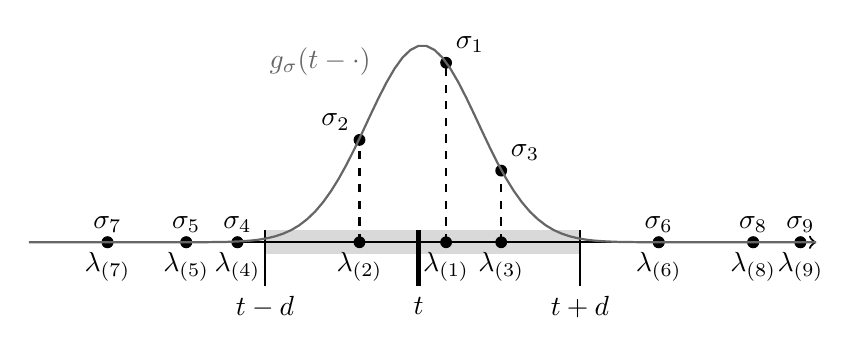
\begin{tikzpicture}
    \fill[black!15!white] (-2.0, -0.15) rectangle (2.0, 0.15);
    \draw[thick, ->] (-5, 0) to (5, 0);
    \fill[black] (-4, 0) circle (0.075) node[below] {$\lambda_{(7)}$};
    \fill[black] (-3, 0) circle (0.075) node[below] {$\lambda_{(5)}$};
    \fill[black] (-2.35, 0) circle (0.075) node[below] {$\lambda_{(4)}$};
    \fill[black] (-0.8, 0) circle (0.075) node[below] {$\lambda_{(2)}$};
    \fill[black] (0.3, 0) circle (0.075) node[below] {$\lambda_{(1)}$};
    \fill[black] (1, 0) circle (0.075) node[below] {$\lambda_{(3)}$};
    \fill[black] (3, 0) circle (0.075) node[below] {$\lambda_{(6)}$};
    \fill[black] (4.2, 0) circle (0.075) node[below] {$\lambda_{(8)}$};
    \fill[black] (4.8, 0) circle (0.075) node[below] {$\lambda_{(9)}$};
    \fill[black] (-4, 0) circle (0.075) node[above] {$\sigma_{7}$};
    \fill[black] (-3, 0) circle (0.075) node[above] {$\sigma_{5}$};
    \fill[black] (-2.35, 0) circle (0.075) node[above] {$\sigma_{4}$};
    \fill[black] (-0.8, 1.3) circle (0.075) node[above left] {$\sigma_{2}$};
    \fill[black] (0.3, 2.28) circle (0.075) node[above right] {$\sigma_{1}$};
    \fill[black] (1, 0.91) circle (0.075) node[above right] {$\sigma_{3}$};
    \fill[black] (3, 0) circle (0.075) node[above] {$\sigma_{6}$};
    \fill[black] (4.2, 0) circle (0.075) node[above] {$\sigma_{8}$};
    \fill[black] (4.8, 0) circle (0.075) node[above] {$\sigma_{9}$};
    \draw[black, ultra thick] (-0.05, 0.15) to (-0.05, -0.55) node[below] {$t$};
    \draw[black, thick] (-2.0, 0.15) to (-2.0, -0.55) node[below] {$t - d$};
    \draw[black, thick] (2.0, 0.15) to (2.0, -0.55) node[below] {$t + d$};
    \draw[black, thick, dashed] (-0.8, 0) to (-0.8, 1.3);
    \draw[black, thick, dashed] (0.3, 0) to (0.3, 2.28);
    \draw[black, thick, dashed] (1, 0) to (1, 0.91);
    \draw[black!60!white, thick] (-5.000, 0.000) to (-4.899, 0.000) to (-4.798, 0.000) to (-4.697, 0.000) to (-4.596, 0.000) to (-4.495, 0.000) to (-4.394, 0.000) to (-4.293, 0.000) to (-4.192, 0.000) to (-4.091, 0.000) to (-3.990, 0.000) to (-3.889, 0.000) to (-3.788, 0.000) to (-3.687, 0.000) to (-3.586, 0.000) to (-3.485, 0.000) to (-3.384, 0.000) to (-3.283, 0.000) to (-3.182, 0.000) to (-3.081, 0.000) to (-2.980, 0.000) to (-2.879, 0.001) to (-2.778, 0.001) to (-2.677, 0.002) to (-2.576, 0.003) to (-2.475, 0.005) to (-2.374, 0.009) to (-2.273, 0.014) to (-2.172, 0.022) to (-2.071, 0.034) to (-1.970, 0.052) to (-1.869, 0.076) to (-1.768, 0.110) to (-1.667, 0.155) to (-1.566, 0.215) to (-1.465, 0.293) to (-1.364, 0.389) to (-1.263, 0.508) to (-1.162, 0.649) to (-1.061, 0.812) to (-0.960, 0.995) to (-0.859, 1.196) to (-0.758, 1.408) to (-0.657, 1.625) to (-0.556, 1.836) to (-0.455, 2.033) to (-0.354, 2.206) to (-0.253, 2.346) to (-0.152, 2.443) to (-0.051, 2.494) to (0.051, 2.494) to (0.152, 2.443) to (0.253, 2.346) to (0.354, 2.206) to (0.455, 2.033) to (0.556, 1.836) to (0.657, 1.625) to (0.758, 1.408) to (0.859, 1.196) to (0.960, 0.995) to (1.061, 0.812) to (1.162, 0.649) to (1.263, 0.508) to (1.364, 0.389) to (1.465, 0.293) to (1.566, 0.215) to (1.667, 0.155) to (1.768, 0.110) to (1.869, 0.076) to (1.970, 0.052) to (2.071, 0.034) to (2.172, 0.022) to (2.273, 0.014) to (2.374, 0.009) to (2.475, 0.005) to (2.576, 0.003) to (2.677, 0.002) to (2.778, 0.001) to (2.879, 0.001) to (2.980, 0.000) to (3.081, 0.000) to (3.182, 0.000) to (3.283, 0.000) to (3.384, 0.000) to (3.485, 0.000) to (3.586, 0.000) to (3.687, 0.000) to (3.788, 0.000) to (3.889, 0.000) to (3.990, 0.000) to (4.091, 0.000) to (4.192, 0.000) to (4.293, 0.000) to (4.394, 0.000) to (4.495, 0.000) to (4.596, 0.000) to (4.697, 0.000) to (4.798, 0.000) to (4.899, 0.000) to (5.000, 0.000);
    \node[black!60!white] at (-1.3, 2.3) {$g_{\sigma}(t - \cdot)$};
\end{tikzpicture}

    \caption{Singular values $\sigma_i$ of $g_{\sigma}(t\mtx{I}_n - \mtx{A})$ corresponding to eigenvalues $\lambda_{(i)}$ of $\mtx{A}$ which lie further away from $t$ than a certain distance $d$ are negligibly small.}
    \label{fig:numerical-rank}
\end{figure}
By choosing $n_{\mtx{\Omega}}$ such that the sum $\sum_{i=n_{\mtx{\Omega}}+5}^{n} \sigma_i(t)$ becomes negligibly small,  \refthm{thm:nystrom} implies an excellent approximation with high probability. In particular, if we assume the eigenvalues of $\mtx{A}$ to be roughly uniformly distributed, a small calculation shows that $n_{\mtx{\Omega}} = \mathcal{O}(n \sigma \sqrt{\log(\varepsilon^{-1}) + \log(\sigma^{-1})})$ will ensure this.


\section{Numerical experiments}
\label{sec:results}


In this section, we verify the performance of the Chebyshev-Nyström++ algorithm proposed in this paper in various application scenarios, from electronic structure interaction, statistical thermodynamics, and neural network optimization.

While theoretically an important tool, we have observed that the preservation of non-negativity discussed in~\refsec{sec:preservnonneg} is not needed in practice. The (slight) indefiniteness of the standard Chebyshev approximation $g_{\sigma}^{(m)}(t \mtx{I}_n - \mtx{A})$ from~\refequ{equ:matrix-approximation} does not seem to impede the reliability of the Nyström++ estimator. Unless otherwise stated, we transform the input matrices such that their eigenvalues are contained in $[-1, 1]$, by approximating their spectrum with NumPy's Hermitian eigenvalue solver before we apply the methods to them. We compute spectral densities at $n_t = 100$ uniformly distributed values of the parameter $t \in [-1, 1]$. The integral involved in computing the $L^1$-errors is approximated with the composite midpoint quadrature rule using the $n_t$ values of $t$ as nodes. Both parameters introduced at the end \refsec{subsubsec:chebyshev-nystrom-implementation},the eigenvalue truncation threshold and the parameter for detecting a vanishing spectral density, are fixed to $10^{-5}$.

Our implementations are written in Python 3.12.3 using the packages NumPy 2.0.0 and SciPy 1.14.1. They are executed on a single thread of a GitHub-hosted Ubuntu runner with a 64-bit processor and 16 GB of RAM. 

\subsection{Spectral density for Hamiltonian of electronic structure}
\label{subsec:hamiltonian}

We use the electronic structure interaction example from~\cite[Section 6]{lin-2017-randomized-estimation}, which involves the second order finite difference discretization of the Hamiltonian
\begin{equation}
    \mathcal{H} = - \Delta + V
    \label{equ:electronic-hamiltonian}
\end{equation}
in three dimensions. The potential $V$ interacting with the electrons is generated by Gaussian wells
    $v(r) = v_0 e^{-\lambda r^2}$, 
with $v_0 = -4$ and $\lambda = 8$, centered in cells of side length $L=6$ which are stacked $n_c \in \mathbb{N}$ times in each spatial dimension; see \reffig{fig:gaussian-well}. The grid width of the finite difference discretization is fixed to $h=0.6$. For $n_c = 1$, this leads to a sparse matrix of size $1\,000 \times 1\,000$ and for $n_c = 2$ of size $8\,000 \times 8\,000$. This example represents an idealized model for the interaction of nuclei on a regular grid with electrons for a $k$-vector in the center of the first Brillouin zone. The distribution of the eigenvalues of the Hamiltonian --- its spectral density --- allows one to interpret the system's energy levels.

\begin{figure}[ht]
    \begin{subfigure}[b]{0.32\columnwidth}
        \input{plots/gaussian-well-1.pgf}
        \caption{$n_c=1$}
        \label{fig:gaussian-well-1}
    \end{subfigure}
    \begin{subfigure}[b]{0.32\columnwidth}
        \input{plots/gaussian-well-2.pgf}
        \caption{$n_c=2$}
        \label{fig:gaussian-well-2}
    \end{subfigure}
    \begin{subfigure}[b]{0.32\columnwidth}
        \input{plots/gaussian-well-5.pgf}
        \caption{$n_c=5$}
        \label{fig:gaussian-well-5}
    \end{subfigure}
    \caption{Cross-sections of the periodic Gaussian wells potential $V$ for different $n_c$.}
    \label{fig:gaussian-well}
\end{figure}

\reffig{fig:convergence} displays the convergence behavior of Chebyshev-Nyström++ applied to the matrix $\mtx{A}$ resulting from the discretization of the Hamiltonian for $n_c = 1$ and $n_c = 2$. Unlike \cite{lin-2017-randomized-estimation}, where just a small portion of the spectral density is considered, we approximate the whole spectrum of $\mtx{A}$ (transformed to $[-1, 1]$) in accordance with our theoretical results (\refsec{subsubsec:chebyshev-nystrom-analysis}) and to demonstrate the effectiveness of our implementational particularities (\refsec{subsubsec:chebyshev-nystrom-implementation}). As a reference, we use the eigenvalues computed by NumPy's Hermitian eigenvalue solver.
\begin{figure}[ht]
    \centering
    \begin{subfigure}[b]{0.495\textwidth}
        \input{plots/convergence-1.pgf}
        \caption{$n_c = 1.$}
        \label{fig:convergence-1}
    \end{subfigure}
    \begin{subfigure}[b]{0.495\textwidth}
        \input{plots/convergence-2.pgf}
        \caption{$n_c = 2.$}
        \label{fig:convergence-2}
    \end{subfigure}
    \caption{Error vs. number of random vectors $n_{\mtx{\Psi}} + n_{\mtx{\Omega}}$ (with fixed $\sigma=0.005$ and $m=2000$) when applying  Chebyshev-Nyström++ to the Hamiltonian matrix from~\refsec{subsec:hamiltonian}.}
    \label{fig:convergence}
\end{figure}%
As expected from \refthm{thm:hutchinson}, Girard-Hutchinson alone ($n_{\mtx{\Omega}} = 0$) requires $n_{\mtx{\Psi}} = \mathcal{O}(\varepsilon^{-2})$ samples to achieve an error of order $\varepsilon$. Because the eigenvalues of the matrix are spread out, we observe the better convergence of the Nyström approximation discussed at the end of \refsec{sec:application} once $n_{\mtx{\Omega}}$ is sufficiently large. At this point, we can observe that the errors stagnate around $10^{-6}$ as a consequence of the error made in the Chebyshev approximation. Due to the higher eigenvalue density of $\mtx{A}$ for $n_c = 2$, the stronger convergence can be observed to kick in later in this case, because a larger $n_{\mtx{\Omega}}$ is needed for a good Nyström approximation. In fact, for $n_c = 5$ the eigenvalue density is so high that to profit from this effect, $n_{\mtx{\Omega}}$ would need to be chosen so large that the computations become unfeasible.

For a fixed budget of $n_{\mtx{\Psi}} + n_{\mtx{\Omega}} = 80$ of random vectors, \reffig{fig:distribution} shows how the value of the smoothing parameter $\sigma$ the choice between Nyström ($n_{\mtx{\Omega}}$) and 
Girard-Hutchinson ($n_{\mtx{\Psi}}$). As expected, for small $\sigma$ the Nyström approximation alone suffices, but 
this is not an effective choice for large $\sigma$. Choosing $n_{\mtx{\Psi}} = n_{\mtx{\Omega}}$ constitutes a good compromise.


\begin{figure}[ht]
    \centering
    
\begin{figure}[ht]
    \centering
    \includegraphics[width=\linewidth]{pics/stats.png}
    \vspace{-7pt}
    \caption{Distribution of the data based on steps in the pipeline
    }
    
    \label{fig:distribution}
    \vspace{-10pt}
    
\end{figure}

    \caption{Error vs. $\sigma$ for a fixed budget of $80$ random vectors 
    when applying  Chebyshev-Nyström++ to the Hamiltonian matrix from~\refsec{subsec:hamiltonian} with $n_c = 1$.
The Chebyshev approximation error is made negligible by setting $m=16 / \sigma$ (see \reflem{lem:non-negative-chebyshev-error}).}
    \label{fig:distribution}
\end{figure}

\subsection{Comparison to Krylov-aware trace estimator}
\label{subsec:krylov-aware}

We notice that the Krylov-aware stochastic trace estimator from \cite[Algorithm 3.1]{chen-2023-krylovaware-stochastic} can also effectively be used in the setting of spectral density approximation. It also samples two Gaussian random matrices $\mtx{\Omega} \in \mathbb{R}^{n \times n_{\mtx{\Omega}}}$ and $\mtx{\Psi} \in \mathbb{R}^{n \times n_{\mtx{\Psi}}}$. $\mtx{\Omega}$. It first runs block Lanczos algorithm on $\mtx{A}$ with starting block $\mtx{\Omega}$ for $r$ iterations with reorthogonalization and subsequently $q$ without. The columns of $\mtx{\Psi}$ are then projected onto the complement of the block Krylov subspace generated by the Lanczos algorithm, and are afterwards used as starting vectors for $r$ iterations of the Lanczos algorithm on $\mtx{A}$. What is remarkable is that all these heavy computations are completely independent of the smoothing kernel $g_{\sigma}$ and the parameter $t$. Further, some algebraic manipulations show that similarly to the stochastic Lanczos quadrature \cite[Section 3]{ubaru-2017-fast-estimation}, we can compress the estimator into a quadrature. Since this quadrature is independent of $g_{\sigma}$ and $t$, it can be applied to different smoothing kernels $g_{\sigma}$ and to as many values of $t$ as needed --- at little additional cost.

We run our own, faithfully optimized implementation of the Krylov-aware stochastic trace estimator \cite[Algorithm 3.1]{chen-2023-krylovaware-stochastic} for different parameter settings on the example from \refsec{subsec:hamiltonian} and plot the approximation errors for logarithmically spaced values of the smoothing parameter $\sigma$ in \reffig{fig:krylov-aware-density}. For reference, we also report the error of Chebyshev-Nyström++ for parameters that lead to a comparable run-time. While the the Krylov-aware estimator is clearly an attractive alternative, it requires a careful choice of parameters adapted to  different regimes of $\sigma$ and still leads to a significantly larger error for moderately small values $\sigma$.

\begin{figure}[ht]
    \begin{minipage}[c]{.475\linewidth}
        \centering
        \input{plots/krylov_aware_density.pgf}
    \end{minipage}\hfill%
    \begin{minipage}[c]{.475\linewidth}
        \vspace{-35pt}
        \centering
\renewcommand{\arraystretch}{1.2}
\begin{tabular}{@{}lccccc@{}}
\toprule
 & $n_{\mtx{\Omega}}$ & $n_{\mtx{\Psi}}$ & $q$ & $r$ & time (s)\\
\midrule
KA (I) & $10$ & $60$ & $20$ & $10$ & $3.17$ \\
KA (II) & $20$ & $30$ & $20$ & $10$ & $1.72$ \\
KA (III) & $10$ & $30$ & $40$ & $10$ & $3.74$ \\
KA (IV) & $10$ & $30$ & $20$ & $20$ & $2.29$ \\
\bottomrule
\end{tabular}

        \newline
        \vspace{15pt}
        \newline
        \centering
\renewcommand{\arraystretch}{1.2}
\begin{tabular}{@{}lcccc@{}}
\toprule
 & $n_{\mtx{\Omega}}$ & $n_{\mtx{\Psi}}$ & $m$ & time (s)\\
\midrule
CN++ & $20$ & $20$ & $2000$ & $3.77$ \\
\bottomrule
\end{tabular}

    \end{minipage}
    \caption{For the example from \refsec{subsec:hamiltonian}, error vs. $\sigma$ the Krylov-Aware (KA) stochastic trace estimator with different parameter settings, compared to the Chebyshev-Nyström++ (CN++) method.}
    \label{fig:krylov-aware-density}
\end{figure}

\subsection{Spectral density of Hessian matrix of neural network}
\label{subsec:hessian}

When fitting the parameters of a neural network, it can be of interest to determine whether a (local) minimum has been found and whether this minimum is robust, i.e., whether a small perturbation of the parameters leads to a significant decrease in the fit of the neural network. Both properties are reflected in the eigenvalues of the Hessian matrix $\mtx{A}$ with respect to some loss function: if all eigenvalues are non-negative, then the loss attains a local minimum, and if, additionally, all of them are small, we talk about a flat minimum; one where small perturbations of the parameters do not cause large increases of the loss and are therefore associated with better generalization \cite{yao-2020-pyhessian-neural}. On the other hand, large eigenvalues in the spectrum indicate high sensitivity of the loss to small changes in the parameters. Those we want to avoid, which is the reason why we monitor them.

Since neural networks are usually parametrized by a large number of parameters, assembling the Hessian matrix explicitly and then computing its eigenvalues is clearly infeasible. On the other hand, one can cheaply compute matrix-vector products $\mtx{A} \vct{x}$ with the Hessian, at a cost that scales proportionally with the number of parameters \cite{pearlmutter-1994-fast-exact}.

To demonstrate that our algorithm can effectively be applied in the setting of neural network optimization, we approximate the spectral density of a small fully connected convolutional neural network with $6\,782$ parameters. We train this network on the handwritten digit classification task given by the MNIST dataset\footnote{Handwritten digit classification; taken from \url{http://yann.lecun.com/exdb/mnist}.} in PyTorch 2.4.1 in a standard way. We use the bound from \cite[Theorem 1]{zhou-2011-bounding-spectrum} to estimate bounds on the spectrum.

We plot the spectral density of the Hessian matrix of the untrained neural network, and at different stages of training in \reffig{fig:hessian-density}, as well as the corresponding mean squared error loss. It can be observed that the eigenvalues creep towards zero as the training proceeds. Furthermore, despite the loss steadily decreasing, the presence of relatively large eigenvalues in some epochs indicates a sharp minimum of the network, hence, unfavorable generalization properties.

\begin{figure}
    \begin{minipage}[c]{.49\linewidth}
        \centering
        \input{plots/hessian_density.pgf}
    \end{minipage}\hfill%
    \begin{minipage}[c]{.49\linewidth}
        \centering
        \input{plots/hessian_density_loss.pgf}
    \end{minipage}
    \caption{Mean squared error training loss (right) and corresponding approximate spectral density of the Hessian matrix of a fully connected convolutional neural network in different epochs of training on the MNIST dataset (left). The spectral density is approximated in $n_t=150$ uniformly spaced points using Chebyshev-Nyström++ with parameters $n_{\mtx{\Omega}} = 10$, $n_{\mtx{\Psi}} = 10$, $m = 1000$, and $\sigma = 0.005$.}
    \label{fig:hessian-density}
\end{figure}

\subsection{Approximation of the partition function of a quantum system}
\label{subsec:spin-chain}

To demonstrate that the Chebyshev-Nyström++ estimator is also effective for problems unrelated to spectral density estimation, we consider the problem of approximating the partition function $\Trace(\exp(-\beta \mtx{A}))$ for the $1\,048\,576 \times 1\,048\,576$ Hamiltonian $\mtx{A}$ of a planar Heisenberg spin chain from~\cite[Section 5.1]{chen-2023-krylovaware-stochastic}. We compute the pointwise error from the analytic solution as a function of the temperature $t\equiv \beta^{-1}$ and compare it to the error achieved by the Krylov-aware trace estimator in \reffig{fig:krylov-aware-spin}.

\begin{figure}[ht]
    \begin{minipage}[c]{.475\linewidth}
        \centering
        \input{plots/krylov_aware_spin.pgf}
    \end{minipage}\hfill%
    \begin{minipage}[c]{.475\linewidth}
        \vspace{-35pt}
        \centering
\renewcommand{\arraystretch}{1.2}
\begin{tabular}{@{}lccccc@{}}
\toprule
 & $n_{\mtx{\Omega}}$ & $n_{\mtx{\Psi}}$ & $q$ & $r$ & time (s)\\
\midrule
KA (i) & $8$ & $0$ & $30$ & $50$ & $9.66$ \\
KA (ii) & $0$ & $13$ & $0$ & $50$ & $4.17$ \\
KA (iii) & $8$ & $13$ & $30$ & $50$ & $17.32$ \\
KA (iv) & $4$ & $6$ & $30$ & $50$ & $8.79$ \\
\bottomrule
\end{tabular}

        \newline
        \vspace{15pt}
        \newline
        \centering
\renewcommand{\arraystretch}{1.2}
\begin{tabular}{@{}lcccc@{}}
\toprule
 & $n_{\mtx{\Omega}}$ & $n_{\mtx{\Psi}}$ & $m$ & time (s)\\
\midrule
CN++ & $40$ & $40$ & $50$ & $23.28$ \\
\bottomrule
\end{tabular}

    \end{minipage}
    \caption{For the Heisenberg spin chain example, we compare the Chebyshev-Nyström++ (CN++) method with the Krylov-Aware stochastic trace estimator in the same configurations as in \cite[Table 5.1]{chen-2023-krylovaware-stochastic} (right). To this extent, we compute the $L^1$-error of the methods for various choices of the temperature parameter $\beta^{-1}$ (left).}
    \label{fig:krylov-aware-spin}
\end{figure}

Unlike for the spectral density example from \refsec{subsec:hamiltonian}, where the numerical rank of the matrix is relatively uniform across different $t$, this now changes changes wildly with the parameter $\beta$. Recall that the Chebyshev-Nyström++ method requires a fixed allocation of random vectors to the low-rank approximation for all values of the parameter $\beta$. Hence, both for large $\beta$, where the matrix $\exp(-\beta \mtx{A})$ has low numerical rank, and for small $\beta$, where the singular values decay very slowly, the approximation error is relatively large. Similarly, one degree $m$ for the Chebyshev approximation needs to be fixed for all $\beta$. Clearly, for large values $\beta$, where $s \mapsto \exp(-\beta s)$ becomes difficult to approximate with polynomials, the fixed degree $m$ is not sufficient for a good Chebyshev approximation, and consequently, the Chebyshev-Nyström++ method is very inaccurate.

\section{Conclusion}
In this work, we propose a simple yet effective approach, called SMILE, for graph few-shot learning with fewer tasks. Specifically, we introduce a novel dual-level mixup strategy, including within-task and across-task mixup, for enriching the diversity of nodes within each task and the diversity of tasks. Also, we incorporate the degree-based prior information to learn expressive node embeddings. Theoretically, we prove that SMILE effectively enhances the model's generalization performance. Empirically, we conduct extensive experiments on multiple benchmarks and the results suggest that SMILE significantly outperforms other baselines, including both in-domain and cross-domain few-shot settings.

\paragraph{Acknowledgements.} The authors gratefully acknowledge the help of Lin Lin in reproducing the example in \refsec{subsec:hamiltonian}. They thank David Persson for many enlightening discussions relating the proof in \refsec{subsec:nystrom-pp}.

\printbibliography

\subsection{Lloyd-Max Algorithm}
\label{subsec:Lloyd-Max}
For a given quantization bitwidth $B$ and an operand $\bm{X}$, the Lloyd-Max algorithm finds $2^B$ quantization levels $\{\hat{x}_i\}_{i=1}^{2^B}$ such that quantizing $\bm{X}$ by rounding each scalar in $\bm{X}$ to the nearest quantization level minimizes the quantization MSE. 

The algorithm starts with an initial guess of quantization levels and then iteratively computes quantization thresholds $\{\tau_i\}_{i=1}^{2^B-1}$ and updates quantization levels $\{\hat{x}_i\}_{i=1}^{2^B}$. Specifically, at iteration $n$, thresholds are set to the midpoints of the previous iteration's levels:
\begin{align*}
    \tau_i^{(n)}=\frac{\hat{x}_i^{(n-1)}+\hat{x}_{i+1}^{(n-1)}}2 \text{ for } i=1\ldots 2^B-1
\end{align*}
Subsequently, the quantization levels are re-computed as conditional means of the data regions defined by the new thresholds:
\begin{align*}
    \hat{x}_i^{(n)}=\mathbb{E}\left[ \bm{X} \big| \bm{X}\in [\tau_{i-1}^{(n)},\tau_i^{(n)}] \right] \text{ for } i=1\ldots 2^B
\end{align*}
where to satisfy boundary conditions we have $\tau_0=-\infty$ and $\tau_{2^B}=\infty$. The algorithm iterates the above steps until convergence.

Figure \ref{fig:lm_quant} compares the quantization levels of a $7$-bit floating point (E3M3) quantizer (left) to a $7$-bit Lloyd-Max quantizer (right) when quantizing a layer of weights from the GPT3-126M model at a per-tensor granularity. As shown, the Lloyd-Max quantizer achieves substantially lower quantization MSE. Further, Table \ref{tab:FP7_vs_LM7} shows the superior perplexity achieved by Lloyd-Max quantizers for bitwidths of $7$, $6$ and $5$. The difference between the quantizers is clear at 5 bits, where per-tensor FP quantization incurs a drastic and unacceptable increase in perplexity, while Lloyd-Max quantization incurs a much smaller increase. Nevertheless, we note that even the optimal Lloyd-Max quantizer incurs a notable ($\sim 1.5$) increase in perplexity due to the coarse granularity of quantization. 

\begin{figure}[h]
  \centering
  \includegraphics[width=0.7\linewidth]{sections/figures/LM7_FP7.pdf}
  \caption{\small Quantization levels and the corresponding quantization MSE of Floating Point (left) vs Lloyd-Max (right) Quantizers for a layer of weights in the GPT3-126M model.}
  \label{fig:lm_quant}
\end{figure}

\begin{table}[h]\scriptsize
\begin{center}
\caption{\label{tab:FP7_vs_LM7} \small Comparing perplexity (lower is better) achieved by floating point quantizers and Lloyd-Max quantizers on a GPT3-126M model for the Wikitext-103 dataset.}
\begin{tabular}{c|cc|c}
\hline
 \multirow{2}{*}{\textbf{Bitwidth}} & \multicolumn{2}{|c|}{\textbf{Floating-Point Quantizer}} & \textbf{Lloyd-Max Quantizer} \\
 & Best Format & Wikitext-103 Perplexity & Wikitext-103 Perplexity \\
\hline
7 & E3M3 & 18.32 & 18.27 \\
6 & E3M2 & 19.07 & 18.51 \\
5 & E4M0 & 43.89 & 19.71 \\
\hline
\end{tabular}
\end{center}
\end{table}

\subsection{Proof of Local Optimality of LO-BCQ}
\label{subsec:lobcq_opt_proof}
For a given block $\bm{b}_j$, the quantization MSE during LO-BCQ can be empirically evaluated as $\frac{1}{L_b}\lVert \bm{b}_j- \bm{\hat{b}}_j\rVert^2_2$ where $\bm{\hat{b}}_j$ is computed from equation (\ref{eq:clustered_quantization_definition}) as $C_{f(\bm{b}_j)}(\bm{b}_j)$. Further, for a given block cluster $\mathcal{B}_i$, we compute the quantization MSE as $\frac{1}{|\mathcal{B}_{i}|}\sum_{\bm{b} \in \mathcal{B}_{i}} \frac{1}{L_b}\lVert \bm{b}- C_i^{(n)}(\bm{b})\rVert^2_2$. Therefore, at the end of iteration $n$, we evaluate the overall quantization MSE $J^{(n)}$ for a given operand $\bm{X}$ composed of $N_c$ block clusters as:
\begin{align*}
    \label{eq:mse_iter_n}
    J^{(n)} = \frac{1}{N_c} \sum_{i=1}^{N_c} \frac{1}{|\mathcal{B}_{i}^{(n)}|}\sum_{\bm{v} \in \mathcal{B}_{i}^{(n)}} \frac{1}{L_b}\lVert \bm{b}- B_i^{(n)}(\bm{b})\rVert^2_2
\end{align*}

At the end of iteration $n$, the codebooks are updated from $\mathcal{C}^{(n-1)}$ to $\mathcal{C}^{(n)}$. However, the mapping of a given vector $\bm{b}_j$ to quantizers $\mathcal{C}^{(n)}$ remains as  $f^{(n)}(\bm{b}_j)$. At the next iteration, during the vector clustering step, $f^{(n+1)}(\bm{b}_j)$ finds new mapping of $\bm{b}_j$ to updated codebooks $\mathcal{C}^{(n)}$ such that the quantization MSE over the candidate codebooks is minimized. Therefore, we obtain the following result for $\bm{b}_j$:
\begin{align*}
\frac{1}{L_b}\lVert \bm{b}_j - C_{f^{(n+1)}(\bm{b}_j)}^{(n)}(\bm{b}_j)\rVert^2_2 \le \frac{1}{L_b}\lVert \bm{b}_j - C_{f^{(n)}(\bm{b}_j)}^{(n)}(\bm{b}_j)\rVert^2_2
\end{align*}

That is, quantizing $\bm{b}_j$ at the end of the block clustering step of iteration $n+1$ results in lower quantization MSE compared to quantizing at the end of iteration $n$. Since this is true for all $\bm{b} \in \bm{X}$, we assert the following:
\begin{equation}
\begin{split}
\label{eq:mse_ineq_1}
    \tilde{J}^{(n+1)} &= \frac{1}{N_c} \sum_{i=1}^{N_c} \frac{1}{|\mathcal{B}_{i}^{(n+1)}|}\sum_{\bm{b} \in \mathcal{B}_{i}^{(n+1)}} \frac{1}{L_b}\lVert \bm{b} - C_i^{(n)}(b)\rVert^2_2 \le J^{(n)}
\end{split}
\end{equation}
where $\tilde{J}^{(n+1)}$ is the the quantization MSE after the vector clustering step at iteration $n+1$.

Next, during the codebook update step (\ref{eq:quantizers_update}) at iteration $n+1$, the per-cluster codebooks $\mathcal{C}^{(n)}$ are updated to $\mathcal{C}^{(n+1)}$ by invoking the Lloyd-Max algorithm \citep{Lloyd}. We know that for any given value distribution, the Lloyd-Max algorithm minimizes the quantization MSE. Therefore, for a given vector cluster $\mathcal{B}_i$ we obtain the following result:

\begin{equation}
    \frac{1}{|\mathcal{B}_{i}^{(n+1)}|}\sum_{\bm{b} \in \mathcal{B}_{i}^{(n+1)}} \frac{1}{L_b}\lVert \bm{b}- C_i^{(n+1)}(\bm{b})\rVert^2_2 \le \frac{1}{|\mathcal{B}_{i}^{(n+1)}|}\sum_{\bm{b} \in \mathcal{B}_{i}^{(n+1)}} \frac{1}{L_b}\lVert \bm{b}- C_i^{(n)}(\bm{b})\rVert^2_2
\end{equation}

The above equation states that quantizing the given block cluster $\mathcal{B}_i$ after updating the associated codebook from $C_i^{(n)}$ to $C_i^{(n+1)}$ results in lower quantization MSE. Since this is true for all the block clusters, we derive the following result: 
\begin{equation}
\begin{split}
\label{eq:mse_ineq_2}
     J^{(n+1)} &= \frac{1}{N_c} \sum_{i=1}^{N_c} \frac{1}{|\mathcal{B}_{i}^{(n+1)}|}\sum_{\bm{b} \in \mathcal{B}_{i}^{(n+1)}} \frac{1}{L_b}\lVert \bm{b}- C_i^{(n+1)}(\bm{b})\rVert^2_2  \le \tilde{J}^{(n+1)}   
\end{split}
\end{equation}

Following (\ref{eq:mse_ineq_1}) and (\ref{eq:mse_ineq_2}), we find that the quantization MSE is non-increasing for each iteration, that is, $J^{(1)} \ge J^{(2)} \ge J^{(3)} \ge \ldots \ge J^{(M)}$ where $M$ is the maximum number of iterations. 
%Therefore, we can say that if the algorithm converges, then it must be that it has converged to a local minimum. 
\hfill $\blacksquare$


\begin{figure}
    \begin{center}
    \includegraphics[width=0.5\textwidth]{sections//figures/mse_vs_iter.pdf}
    \end{center}
    \caption{\small NMSE vs iterations during LO-BCQ compared to other block quantization proposals}
    \label{fig:nmse_vs_iter}
\end{figure}

Figure \ref{fig:nmse_vs_iter} shows the empirical convergence of LO-BCQ across several block lengths and number of codebooks. Also, the MSE achieved by LO-BCQ is compared to baselines such as MXFP and VSQ. As shown, LO-BCQ converges to a lower MSE than the baselines. Further, we achieve better convergence for larger number of codebooks ($N_c$) and for a smaller block length ($L_b$), both of which increase the bitwidth of BCQ (see Eq \ref{eq:bitwidth_bcq}).


\subsection{Additional Accuracy Results}
%Table \ref{tab:lobcq_config} lists the various LOBCQ configurations and their corresponding bitwidths.
\begin{table}
\setlength{\tabcolsep}{4.75pt}
\begin{center}
\caption{\label{tab:lobcq_config} Various LO-BCQ configurations and their bitwidths.}
\begin{tabular}{|c||c|c|c|c||c|c||c|} 
\hline
 & \multicolumn{4}{|c||}{$L_b=8$} & \multicolumn{2}{|c||}{$L_b=4$} & $L_b=2$ \\
 \hline
 \backslashbox{$L_A$\kern-1em}{\kern-1em$N_c$} & 2 & 4 & 8 & 16 & 2 & 4 & 2 \\
 \hline
 64 & 4.25 & 4.375 & 4.5 & 4.625 & 4.375 & 4.625 & 4.625\\
 \hline
 32 & 4.375 & 4.5 & 4.625& 4.75 & 4.5 & 4.75 & 4.75 \\
 \hline
 16 & 4.625 & 4.75& 4.875 & 5 & 4.75 & 5 & 5 \\
 \hline
\end{tabular}
\end{center}
\end{table}

%\subsection{Perplexity achieved by various LO-BCQ configurations on Wikitext-103 dataset}

\begin{table} \centering
\begin{tabular}{|c||c|c|c|c||c|c||c|} 
\hline
 $L_b \rightarrow$& \multicolumn{4}{c||}{8} & \multicolumn{2}{c||}{4} & 2\\
 \hline
 \backslashbox{$L_A$\kern-1em}{\kern-1em$N_c$} & 2 & 4 & 8 & 16 & 2 & 4 & 2  \\
 %$N_c \rightarrow$ & 2 & 4 & 8 & 16 & 2 & 4 & 2 \\
 \hline
 \hline
 \multicolumn{8}{c}{GPT3-1.3B (FP32 PPL = 9.98)} \\ 
 \hline
 \hline
 64 & 10.40 & 10.23 & 10.17 & 10.15 &  10.28 & 10.18 & 10.19 \\
 \hline
 32 & 10.25 & 10.20 & 10.15 & 10.12 &  10.23 & 10.17 & 10.17 \\
 \hline
 16 & 10.22 & 10.16 & 10.10 & 10.09 &  10.21 & 10.14 & 10.16 \\
 \hline
  \hline
 \multicolumn{8}{c}{GPT3-8B (FP32 PPL = 7.38)} \\ 
 \hline
 \hline
 64 & 7.61 & 7.52 & 7.48 &  7.47 &  7.55 &  7.49 & 7.50 \\
 \hline
 32 & 7.52 & 7.50 & 7.46 &  7.45 &  7.52 &  7.48 & 7.48  \\
 \hline
 16 & 7.51 & 7.48 & 7.44 &  7.44 &  7.51 &  7.49 & 7.47  \\
 \hline
\end{tabular}
\caption{\label{tab:ppl_gpt3_abalation} Wikitext-103 perplexity across GPT3-1.3B and 8B models.}
\end{table}

\begin{table} \centering
\begin{tabular}{|c||c|c|c|c||} 
\hline
 $L_b \rightarrow$& \multicolumn{4}{c||}{8}\\
 \hline
 \backslashbox{$L_A$\kern-1em}{\kern-1em$N_c$} & 2 & 4 & 8 & 16 \\
 %$N_c \rightarrow$ & 2 & 4 & 8 & 16 & 2 & 4 & 2 \\
 \hline
 \hline
 \multicolumn{5}{|c|}{Llama2-7B (FP32 PPL = 5.06)} \\ 
 \hline
 \hline
 64 & 5.31 & 5.26 & 5.19 & 5.18  \\
 \hline
 32 & 5.23 & 5.25 & 5.18 & 5.15  \\
 \hline
 16 & 5.23 & 5.19 & 5.16 & 5.14  \\
 \hline
 \multicolumn{5}{|c|}{Nemotron4-15B (FP32 PPL = 5.87)} \\ 
 \hline
 \hline
 64  & 6.3 & 6.20 & 6.13 & 6.08  \\
 \hline
 32  & 6.24 & 6.12 & 6.07 & 6.03  \\
 \hline
 16  & 6.12 & 6.14 & 6.04 & 6.02  \\
 \hline
 \multicolumn{5}{|c|}{Nemotron4-340B (FP32 PPL = 3.48)} \\ 
 \hline
 \hline
 64 & 3.67 & 3.62 & 3.60 & 3.59 \\
 \hline
 32 & 3.63 & 3.61 & 3.59 & 3.56 \\
 \hline
 16 & 3.61 & 3.58 & 3.57 & 3.55 \\
 \hline
\end{tabular}
\caption{\label{tab:ppl_llama7B_nemo15B} Wikitext-103 perplexity compared to FP32 baseline in Llama2-7B and Nemotron4-15B, 340B models}
\end{table}

%\subsection{Perplexity achieved by various LO-BCQ configurations on MMLU dataset}


\begin{table} \centering
\begin{tabular}{|c||c|c|c|c||c|c|c|c|} 
\hline
 $L_b \rightarrow$& \multicolumn{4}{c||}{8} & \multicolumn{4}{c||}{8}\\
 \hline
 \backslashbox{$L_A$\kern-1em}{\kern-1em$N_c$} & 2 & 4 & 8 & 16 & 2 & 4 & 8 & 16  \\
 %$N_c \rightarrow$ & 2 & 4 & 8 & 16 & 2 & 4 & 2 \\
 \hline
 \hline
 \multicolumn{5}{|c|}{Llama2-7B (FP32 Accuracy = 45.8\%)} & \multicolumn{4}{|c|}{Llama2-70B (FP32 Accuracy = 69.12\%)} \\ 
 \hline
 \hline
 64 & 43.9 & 43.4 & 43.9 & 44.9 & 68.07 & 68.27 & 68.17 & 68.75 \\
 \hline
 32 & 44.5 & 43.8 & 44.9 & 44.5 & 68.37 & 68.51 & 68.35 & 68.27  \\
 \hline
 16 & 43.9 & 42.7 & 44.9 & 45 & 68.12 & 68.77 & 68.31 & 68.59  \\
 \hline
 \hline
 \multicolumn{5}{|c|}{GPT3-22B (FP32 Accuracy = 38.75\%)} & \multicolumn{4}{|c|}{Nemotron4-15B (FP32 Accuracy = 64.3\%)} \\ 
 \hline
 \hline
 64 & 36.71 & 38.85 & 38.13 & 38.92 & 63.17 & 62.36 & 63.72 & 64.09 \\
 \hline
 32 & 37.95 & 38.69 & 39.45 & 38.34 & 64.05 & 62.30 & 63.8 & 64.33  \\
 \hline
 16 & 38.88 & 38.80 & 38.31 & 38.92 & 63.22 & 63.51 & 63.93 & 64.43  \\
 \hline
\end{tabular}
\caption{\label{tab:mmlu_abalation} Accuracy on MMLU dataset across GPT3-22B, Llama2-7B, 70B and Nemotron4-15B models.}
\end{table}


%\subsection{Perplexity achieved by various LO-BCQ configurations on LM evaluation harness}

\begin{table} \centering
\begin{tabular}{|c||c|c|c|c||c|c|c|c|} 
\hline
 $L_b \rightarrow$& \multicolumn{4}{c||}{8} & \multicolumn{4}{c||}{8}\\
 \hline
 \backslashbox{$L_A$\kern-1em}{\kern-1em$N_c$} & 2 & 4 & 8 & 16 & 2 & 4 & 8 & 16  \\
 %$N_c \rightarrow$ & 2 & 4 & 8 & 16 & 2 & 4 & 2 \\
 \hline
 \hline
 \multicolumn{5}{|c|}{Race (FP32 Accuracy = 37.51\%)} & \multicolumn{4}{|c|}{Boolq (FP32 Accuracy = 64.62\%)} \\ 
 \hline
 \hline
 64 & 36.94 & 37.13 & 36.27 & 37.13 & 63.73 & 62.26 & 63.49 & 63.36 \\
 \hline
 32 & 37.03 & 36.36 & 36.08 & 37.03 & 62.54 & 63.51 & 63.49 & 63.55  \\
 \hline
 16 & 37.03 & 37.03 & 36.46 & 37.03 & 61.1 & 63.79 & 63.58 & 63.33  \\
 \hline
 \hline
 \multicolumn{5}{|c|}{Winogrande (FP32 Accuracy = 58.01\%)} & \multicolumn{4}{|c|}{Piqa (FP32 Accuracy = 74.21\%)} \\ 
 \hline
 \hline
 64 & 58.17 & 57.22 & 57.85 & 58.33 & 73.01 & 73.07 & 73.07 & 72.80 \\
 \hline
 32 & 59.12 & 58.09 & 57.85 & 58.41 & 73.01 & 73.94 & 72.74 & 73.18  \\
 \hline
 16 & 57.93 & 58.88 & 57.93 & 58.56 & 73.94 & 72.80 & 73.01 & 73.94  \\
 \hline
\end{tabular}
\caption{\label{tab:mmlu_abalation} Accuracy on LM evaluation harness tasks on GPT3-1.3B model.}
\end{table}

\begin{table} \centering
\begin{tabular}{|c||c|c|c|c||c|c|c|c|} 
\hline
 $L_b \rightarrow$& \multicolumn{4}{c||}{8} & \multicolumn{4}{c||}{8}\\
 \hline
 \backslashbox{$L_A$\kern-1em}{\kern-1em$N_c$} & 2 & 4 & 8 & 16 & 2 & 4 & 8 & 16  \\
 %$N_c \rightarrow$ & 2 & 4 & 8 & 16 & 2 & 4 & 2 \\
 \hline
 \hline
 \multicolumn{5}{|c|}{Race (FP32 Accuracy = 41.34\%)} & \multicolumn{4}{|c|}{Boolq (FP32 Accuracy = 68.32\%)} \\ 
 \hline
 \hline
 64 & 40.48 & 40.10 & 39.43 & 39.90 & 69.20 & 68.41 & 69.45 & 68.56 \\
 \hline
 32 & 39.52 & 39.52 & 40.77 & 39.62 & 68.32 & 67.43 & 68.17 & 69.30  \\
 \hline
 16 & 39.81 & 39.71 & 39.90 & 40.38 & 68.10 & 66.33 & 69.51 & 69.42  \\
 \hline
 \hline
 \multicolumn{5}{|c|}{Winogrande (FP32 Accuracy = 67.88\%)} & \multicolumn{4}{|c|}{Piqa (FP32 Accuracy = 78.78\%)} \\ 
 \hline
 \hline
 64 & 66.85 & 66.61 & 67.72 & 67.88 & 77.31 & 77.42 & 77.75 & 77.64 \\
 \hline
 32 & 67.25 & 67.72 & 67.72 & 67.00 & 77.31 & 77.04 & 77.80 & 77.37  \\
 \hline
 16 & 68.11 & 68.90 & 67.88 & 67.48 & 77.37 & 78.13 & 78.13 & 77.69  \\
 \hline
\end{tabular}
\caption{\label{tab:mmlu_abalation} Accuracy on LM evaluation harness tasks on GPT3-8B model.}
\end{table}

\begin{table} \centering
\begin{tabular}{|c||c|c|c|c||c|c|c|c|} 
\hline
 $L_b \rightarrow$& \multicolumn{4}{c||}{8} & \multicolumn{4}{c||}{8}\\
 \hline
 \backslashbox{$L_A$\kern-1em}{\kern-1em$N_c$} & 2 & 4 & 8 & 16 & 2 & 4 & 8 & 16  \\
 %$N_c \rightarrow$ & 2 & 4 & 8 & 16 & 2 & 4 & 2 \\
 \hline
 \hline
 \multicolumn{5}{|c|}{Race (FP32 Accuracy = 40.67\%)} & \multicolumn{4}{|c|}{Boolq (FP32 Accuracy = 76.54\%)} \\ 
 \hline
 \hline
 64 & 40.48 & 40.10 & 39.43 & 39.90 & 75.41 & 75.11 & 77.09 & 75.66 \\
 \hline
 32 & 39.52 & 39.52 & 40.77 & 39.62 & 76.02 & 76.02 & 75.96 & 75.35  \\
 \hline
 16 & 39.81 & 39.71 & 39.90 & 40.38 & 75.05 & 73.82 & 75.72 & 76.09  \\
 \hline
 \hline
 \multicolumn{5}{|c|}{Winogrande (FP32 Accuracy = 70.64\%)} & \multicolumn{4}{|c|}{Piqa (FP32 Accuracy = 79.16\%)} \\ 
 \hline
 \hline
 64 & 69.14 & 70.17 & 70.17 & 70.56 & 78.24 & 79.00 & 78.62 & 78.73 \\
 \hline
 32 & 70.96 & 69.69 & 71.27 & 69.30 & 78.56 & 79.49 & 79.16 & 78.89  \\
 \hline
 16 & 71.03 & 69.53 & 69.69 & 70.40 & 78.13 & 79.16 & 79.00 & 79.00  \\
 \hline
\end{tabular}
\caption{\label{tab:mmlu_abalation} Accuracy on LM evaluation harness tasks on GPT3-22B model.}
\end{table}

\begin{table} \centering
\begin{tabular}{|c||c|c|c|c||c|c|c|c|} 
\hline
 $L_b \rightarrow$& \multicolumn{4}{c||}{8} & \multicolumn{4}{c||}{8}\\
 \hline
 \backslashbox{$L_A$\kern-1em}{\kern-1em$N_c$} & 2 & 4 & 8 & 16 & 2 & 4 & 8 & 16  \\
 %$N_c \rightarrow$ & 2 & 4 & 8 & 16 & 2 & 4 & 2 \\
 \hline
 \hline
 \multicolumn{5}{|c|}{Race (FP32 Accuracy = 44.4\%)} & \multicolumn{4}{|c|}{Boolq (FP32 Accuracy = 79.29\%)} \\ 
 \hline
 \hline
 64 & 42.49 & 42.51 & 42.58 & 43.45 & 77.58 & 77.37 & 77.43 & 78.1 \\
 \hline
 32 & 43.35 & 42.49 & 43.64 & 43.73 & 77.86 & 75.32 & 77.28 & 77.86  \\
 \hline
 16 & 44.21 & 44.21 & 43.64 & 42.97 & 78.65 & 77 & 76.94 & 77.98  \\
 \hline
 \hline
 \multicolumn{5}{|c|}{Winogrande (FP32 Accuracy = 69.38\%)} & \multicolumn{4}{|c|}{Piqa (FP32 Accuracy = 78.07\%)} \\ 
 \hline
 \hline
 64 & 68.9 & 68.43 & 69.77 & 68.19 & 77.09 & 76.82 & 77.09 & 77.86 \\
 \hline
 32 & 69.38 & 68.51 & 68.82 & 68.90 & 78.07 & 76.71 & 78.07 & 77.86  \\
 \hline
 16 & 69.53 & 67.09 & 69.38 & 68.90 & 77.37 & 77.8 & 77.91 & 77.69  \\
 \hline
\end{tabular}
\caption{\label{tab:mmlu_abalation} Accuracy on LM evaluation harness tasks on Llama2-7B model.}
\end{table}

\begin{table} \centering
\begin{tabular}{|c||c|c|c|c||c|c|c|c|} 
\hline
 $L_b \rightarrow$& \multicolumn{4}{c||}{8} & \multicolumn{4}{c||}{8}\\
 \hline
 \backslashbox{$L_A$\kern-1em}{\kern-1em$N_c$} & 2 & 4 & 8 & 16 & 2 & 4 & 8 & 16  \\
 %$N_c \rightarrow$ & 2 & 4 & 8 & 16 & 2 & 4 & 2 \\
 \hline
 \hline
 \multicolumn{5}{|c|}{Race (FP32 Accuracy = 48.8\%)} & \multicolumn{4}{|c|}{Boolq (FP32 Accuracy = 85.23\%)} \\ 
 \hline
 \hline
 64 & 49.00 & 49.00 & 49.28 & 48.71 & 82.82 & 84.28 & 84.03 & 84.25 \\
 \hline
 32 & 49.57 & 48.52 & 48.33 & 49.28 & 83.85 & 84.46 & 84.31 & 84.93  \\
 \hline
 16 & 49.85 & 49.09 & 49.28 & 48.99 & 85.11 & 84.46 & 84.61 & 83.94  \\
 \hline
 \hline
 \multicolumn{5}{|c|}{Winogrande (FP32 Accuracy = 79.95\%)} & \multicolumn{4}{|c|}{Piqa (FP32 Accuracy = 81.56\%)} \\ 
 \hline
 \hline
 64 & 78.77 & 78.45 & 78.37 & 79.16 & 81.45 & 80.69 & 81.45 & 81.5 \\
 \hline
 32 & 78.45 & 79.01 & 78.69 & 80.66 & 81.56 & 80.58 & 81.18 & 81.34  \\
 \hline
 16 & 79.95 & 79.56 & 79.79 & 79.72 & 81.28 & 81.66 & 81.28 & 80.96  \\
 \hline
\end{tabular}
\caption{\label{tab:mmlu_abalation} Accuracy on LM evaluation harness tasks on Llama2-70B model.}
\end{table}

%\section{MSE Studies}
%\textcolor{red}{TODO}


\subsection{Number Formats and Quantization Method}
\label{subsec:numFormats_quantMethod}
\subsubsection{Integer Format}
An $n$-bit signed integer (INT) is typically represented with a 2s-complement format \citep{yao2022zeroquant,xiao2023smoothquant,dai2021vsq}, where the most significant bit denotes the sign.

\subsubsection{Floating Point Format}
An $n$-bit signed floating point (FP) number $x$ comprises of a 1-bit sign ($x_{\mathrm{sign}}$), $B_m$-bit mantissa ($x_{\mathrm{mant}}$) and $B_e$-bit exponent ($x_{\mathrm{exp}}$) such that $B_m+B_e=n-1$. The associated constant exponent bias ($E_{\mathrm{bias}}$) is computed as $(2^{{B_e}-1}-1)$. We denote this format as $E_{B_e}M_{B_m}$.  

\subsubsection{Quantization Scheme}
\label{subsec:quant_method}
A quantization scheme dictates how a given unquantized tensor is converted to its quantized representation. We consider FP formats for the purpose of illustration. Given an unquantized tensor $\bm{X}$ and an FP format $E_{B_e}M_{B_m}$, we first, we compute the quantization scale factor $s_X$ that maps the maximum absolute value of $\bm{X}$ to the maximum quantization level of the $E_{B_e}M_{B_m}$ format as follows:
\begin{align}
\label{eq:sf}
    s_X = \frac{\mathrm{max}(|\bm{X}|)}{\mathrm{max}(E_{B_e}M_{B_m})}
\end{align}
In the above equation, $|\cdot|$ denotes the absolute value function.

Next, we scale $\bm{X}$ by $s_X$ and quantize it to $\hat{\bm{X}}$ by rounding it to the nearest quantization level of $E_{B_e}M_{B_m}$ as:

\begin{align}
\label{eq:tensor_quant}
    \hat{\bm{X}} = \text{round-to-nearest}\left(\frac{\bm{X}}{s_X}, E_{B_e}M_{B_m}\right)
\end{align}

We perform dynamic max-scaled quantization \citep{wu2020integer}, where the scale factor $s$ for activations is dynamically computed during runtime.

\subsection{Vector Scaled Quantization}
\begin{wrapfigure}{r}{0.35\linewidth}
  \centering
  \includegraphics[width=\linewidth]{sections/figures/vsquant.jpg}
  \caption{\small Vectorwise decomposition for per-vector scaled quantization (VSQ \citep{dai2021vsq}).}
  \label{fig:vsquant}
\end{wrapfigure}
During VSQ \citep{dai2021vsq}, the operand tensors are decomposed into 1D vectors in a hardware friendly manner as shown in Figure \ref{fig:vsquant}. Since the decomposed tensors are used as operands in matrix multiplications during inference, it is beneficial to perform this decomposition along the reduction dimension of the multiplication. The vectorwise quantization is performed similar to tensorwise quantization described in Equations \ref{eq:sf} and \ref{eq:tensor_quant}, where a scale factor $s_v$ is required for each vector $\bm{v}$ that maps the maximum absolute value of that vector to the maximum quantization level. While smaller vector lengths can lead to larger accuracy gains, the associated memory and computational overheads due to the per-vector scale factors increases. To alleviate these overheads, VSQ \citep{dai2021vsq} proposed a second level quantization of the per-vector scale factors to unsigned integers, while MX \citep{rouhani2023shared} quantizes them to integer powers of 2 (denoted as $2^{INT}$).

\subsubsection{MX Format}
The MX format proposed in \citep{rouhani2023microscaling} introduces the concept of sub-block shifting. For every two scalar elements of $b$-bits each, there is a shared exponent bit. The value of this exponent bit is determined through an empirical analysis that targets minimizing quantization MSE. We note that the FP format $E_{1}M_{b}$ is strictly better than MX from an accuracy perspective since it allocates a dedicated exponent bit to each scalar as opposed to sharing it across two scalars. Therefore, we conservatively bound the accuracy of a $b+2$-bit signed MX format with that of a $E_{1}M_{b}$ format in our comparisons. For instance, we use E1M2 format as a proxy for MX4.

\begin{figure}
    \centering
    \includegraphics[width=1\linewidth]{sections//figures/BlockFormats.pdf}
    \caption{\small Comparing LO-BCQ to MX format.}
    \label{fig:block_formats}
\end{figure}

Figure \ref{fig:block_formats} compares our $4$-bit LO-BCQ block format to MX \citep{rouhani2023microscaling}. As shown, both LO-BCQ and MX decompose a given operand tensor into block arrays and each block array into blocks. Similar to MX, we find that per-block quantization ($L_b < L_A$) leads to better accuracy due to increased flexibility. While MX achieves this through per-block $1$-bit micro-scales, we associate a dedicated codebook to each block through a per-block codebook selector. Further, MX quantizes the per-block array scale-factor to E8M0 format without per-tensor scaling. In contrast during LO-BCQ, we find that per-tensor scaling combined with quantization of per-block array scale-factor to E4M3 format results in superior inference accuracy across models. 


\end{document}
